\documentclass[12pt, twoside, openany]{report}
\usepackage{graphicx}
\usepackage{a4wide}
\usepackage[utf8]{inputenc}
\usepackage{enumerate}
\usepackage{verbatim}
\usepackage[polish,british]{babel}
\usepackage[T1]{fontenc}
\usepackage{geometry}
\geometry{left=25mm,right=25mm, top=25mm, bottom=25mm}
\usepackage{latexsym}
\usepackage{amsthm}
\usepackage{palatino}
\usepackage{array}
\usepackage{csquotes}
\usepackage{times}
\usepackage{helvet}
\usepackage{textcomp}
\theoremstyle{definition}
\usepackage{perpage} %the perpage package
\MakePerPage{footnote} %the perpage package command
\setcounter{tocdepth}{1}
\newcommand*{\norm}[1]{\left\Vert{#1}\right\Vert}
\newcommand*{\abs}[1]{\left\vert{#1}\right\vert}
\newcommand*{\om}{\omega}



\author{Paweł Paczuski}
\title{Structured radiological reporting system}

\begin{document}
\fontfamily{phv}\selectfont


% Zażółć gęślą jaźń.
\begin{titlepage}
\pagestyle{empty}

\noindent

\includegraphics{title}
\begin{center}
Institute of Computer Science
\end{center}



\includegraphics{bachelor}
\begin{center}
	In the field of study Computer Science  \\

	and specialization Computer Systems and Networks \\
\end{center}

\begin{center}
\large
Structured radiological reporting system\\
\normalsize
\end{center}
\vskip 36pt
\begin{center}
\LARGE
Paweł Paczuski\\
\normalsize
student record book number 271082
\end{center}
\vskip 60pt
\begin{center}
thesis supervisor \\
 Jan J. Mulawka PhD, DSc
\end{center}
\vfill
\begin{center}
\normalsize
WARSAW 2018
\end{center}
\newpage
\hfill


% \maketitle
\end{titlepage}

\fontfamily{ptm}\selectfont

\thispagestyle{empty}
\newpage
\pagestyle{headings}
\setcounter{page}{1}
\hyphenation{Syl-ves-tra}
\hyphenation{Syl-ves-ter-a}
\begin{otherlanguage}{british}
\begin{abstract}
Structured radiological reporting system.

Design and implementation of a system that can be used by radiologists to create structured radiological reports. The system uses sets of standardized, frequently used phrases to: describe state of patient's body captured by other medical diagnostics methods, provide set of tools that minimize risk of mistake and increase productivity. 
\end{abstract}
\end{otherlanguage}
\begin{otherlanguage}{polish}
\begin{abstract}
streszczenie po polsku
\end{abstract}
\end{otherlanguage}

%-----------Początek części zasadniczej-----------
\tableofcontents
\clearpage







\chapter{Introduction}
\section{The need for medical diagnostics}
Everyday millions of physicians treat injuries and illnesses of different kids. Before a doctor can plan an individual treatment for a patient, they have to diagnose which organs are in pathological states \cite{bls}. This sometimes can be achieved by simply glancing at the body, however, there are many illnesses that require specialized set of tools and methods in order to observe which parts of patient's body are in an unwanted state. Through years of research, many different techniques were established and a separate specialization emerged -- radiology. Radiologists focus mainly on analyzing and interpreting diagnostic imagery and as a result of their work they create a document called radiological report which contains description of what can be observed in the image of patient body. Reports may contain description of state of particular organs, measurements (e.g. radius, volume, concentration of certain substances in the blood), comparison of medical condition of a patient observed at different times and description of overall state of the patient. \\
\section{Existing solutions}
Currently, the research is focused on finding new ways of diagnosing diseases by  the use of more advanced equipment or brilliant algorithms that try to automate image analysis \cite{ai}. \\
On the other hand, there exist initiatives that try to improve quality of the radiological reports themselves. There are groups consisting of both computer scientists and physicians that try to standardize reports, prepare checklists that require doctors to describe patients' state in particular order and create a set of phrases that will be understood in the same way by all physicians \cite{snomed}. A lot of work has been done to provide both common medical nomenclature for medical conditions and theoretical framework to describe relations between causes and effects of patients' condition. As there are more and more methods used to diagnose, the amount of information captured increases, so the reporting methodology has to be kept up to date with the state of art. This is why a very specific field -- Structural Reporting (SR) emerged. The basic idea is to provide a way to create radiological reports that conveys as much semantics as possible in a way that is easy to understand. One can find great ideas implemented in such standards as SNOMED SR \cite{sr} and also HL7 version 3 Clinical Document Architecture (HL7 V3 CDA). By using these standards, one can encode relations between organs and diseases (causality) in a very regular format. After encoding structure in the report, one can use algorithms to e.g. highlight what changed since last visit, look for diseases that were diagnosed in the specified time range etc. This is very difficult to achieve when reports are stored in plain text. Structural reporting focuses mainly on encoding meaning -- the visual representation of resulting reports is a separate matter that is treated as an implementation detail \cite{sr}.
In spite of the existence of these standards, it is almost impossible to find software that implements structural reporting techniques. One of the most important reasons is the fact that in order to understand benefits of SR, one has to acquire certain level of understanding of the typical work-flow of a radiologist. As there is huge demand for software that is much easier to understand (e.g. RIS and HIS software), most of the effort is made to implement simpler concepts.

\section{Typical work-flow of a radiologist in Poland}
In order to find places where optimization of productivity could be applied, one has to get to know how a radiologist works and what are activities that waste significant amounts of time. \\
In a medium-sized clinic, medical imagery is captured by a radiologic technologist who then uploads the data to the Picture Archiving and Communication System (PACS) and attaches identification information to the images. Next to the PACS system in most cases exists Radiology Information System (RIS) that is used by radiological staff to keep track of patients treated in the clinic. These systems are used to distribute imagery to the team of radiologists.

Imagery can be distributed in one of the following manners:
\begin{itemize}
    \item Particular patient is always serviced by the same radiologist.
    \item RIS system acts as an accumulator of service requests and radiologist decides which patient they should focus on now.
    \item Certain types of medical examinations are always assigned to a radiologist that is specialized in describing them.
\end{itemize}

After receiving diagnostic imagery, a radiologist uses special software called Viewer\cite{viewer} to navigate through images, make measurements by using visual tools like virtual ruler and examine what is the state of patient's body. Figure \ref{fig:osirix} shows an example of the Viewer software. In parallel to this, the doctor uses text editor and describes what he or she sees in the images. Some RIS systems are equipped with a simple text editors that allow doctors to write the report inside the system without using external editors. 

\begin{figure}
    \centering
    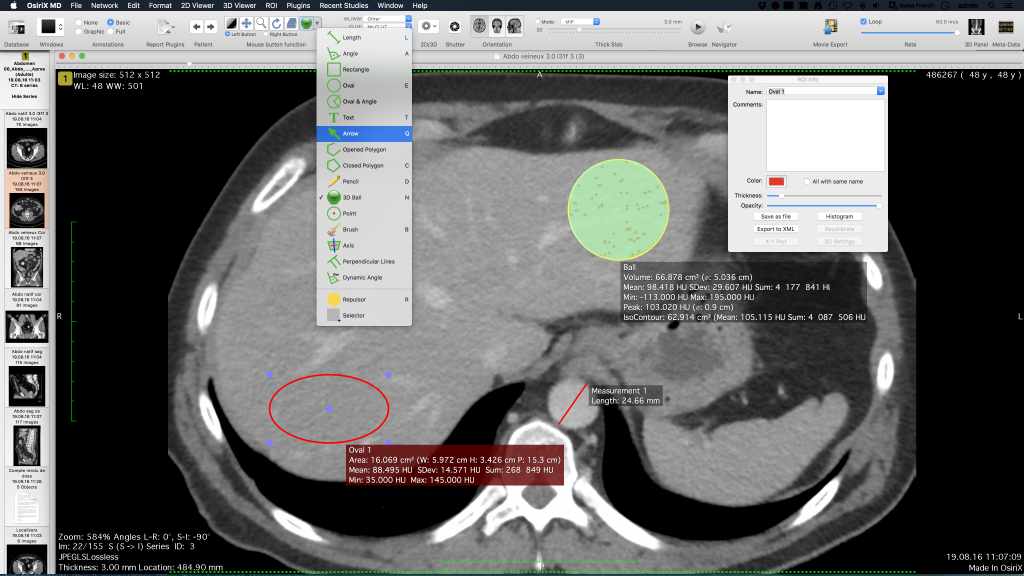
\includegraphics[width=0.9\linewidth]{osirix}
    \caption{OsiriX is one of the most popular image viewers used by the radiologists}
    \label{fig:osirix}
\end{figure}

\section{Discussion about presented work-flow}
\subsection{The good parts}
\subsubsection{Viewer software provides expected functionality}
Viewer software has a very stable position on the market and is perfectly tailored to the needs of a radiologist. It often uses advanced techniques of computer graphics to present patient's body as accurately as possible.
\subsubsection{PACS systems provide centralized place for storing images}
They implement functionalities that allow for archiving medical imagery. Lifetime of medical images is controlled by the government and these systems must take this into account. PACS also make it easy to distribute images not only withing local networks but also to any doctor who has the remote access granted.  
\subsubsection{RIS systems make it easy to exchange data between physicians}
There is no need need for the radiologist to deliver the radiological report to the other physician personally as it is done automatically. Also, RIS systems provide good means of presenting medical records from different medical specializations allowing for interdisciplinary diagnostics. 
\subsection{The bad parts}
\subsubsection{Focus on text rather than semantics}
It is expected that the radiologist will produce a consistent, ordered report by means of text editors. Some RIS systems provide basic text formatting functionality like italicization, underlining but they are limited to the textual presentation of the report. There are no dedicated tools to encode relations in this representation.
\subsubsection{Each radiologist has their own style of writing}
Usually there are no structural expectations about the resulting report. Each radiologist can have their own style of writing, order of organs observation, text formatting. This leads to the waste of time as people who read the report have to make some effort to infer the meaning from plaintext. 
\subsubsection{Selective description}
It is very frequent that radiologists include in the report only things that they consider bad for the patient. This makes the report more goal-oriented but it means that it is useless to get to know the overall state of patient body.
\subsubsection{Copy-paste}
Radiologists try to solve the problem of typing on their own by creating templates that contain certain pathologies listed and what they do is execution of the commonly called 'copy-paste' method to create report content. Sometimes they do not notice parts of copied text that are different from the actual state of the body, so the reports may contain observations that are false. 

\section{Other ways to create radiological reports}
In many English-speaking countries the work-flow of a radiologist differs in the way the radiological report is generated. A radiologist may record their voice while describing the imagery vocally. The recordings are then transcribed using either speech recognition algorithms or manually by technologists. Having a good skill of typing by a radiologist is not required, only knowledge to interpret imagery is used. This approach, however, has some architectural disadvantages. More personnel are needed -- technologists, who transcribe the recorded voice \cite{speech-impact}. Also, it is difficult to make changes to what has been said. In some cases, a mistake can be made while transcribing the text \cite{speech-africa}.

\section{Problem definition}

After analyzing bad parts of the presented work-flow and general situation on the market -- demand for radiological services increases but the number of radiologists appears to be constant, it was decided to design and implement a system that would be used by radiologists to encode semantics of diagnostic imagery in a form that can be easily transformed to the human readable form, analyzed by algorithms. 

\section{Incentives for the thesis}
A primary goal is to find a solution to the problem of not satisfactory productivity of radiologists by implementing a program used to create structured radiological reports. The system should apply sets of standardized, frequently used phrases to: describe state of patient's body captured by other medical diagnostics methods and should also provide set of tools that minimize risk of mistake and allows radiologists to create reports faster. 



\chapter{Description of the proposed solution}
\section{General idea}
\subsection{Area of interest}
The system that is proposed in this thesis focuses entirely on the part of the typical radiological work-flow in which a radiologist focuses on the textual description of what can be seen in the diagnostic imagery.
\subsection{Contextual suggestions}
Several hundreds of anonymized radiological reports have been analyzed and it was observed that a lot of time could be saved, if a radiologist would at any time select text fragments from a predefined set of possibilities that are appropriate to the current context. This approach can be similar to the way Integrated Development Environment (IDE) for statically typed languages (e.g. Visual Studio supporting C\#) are suggesting what the programmer can type based on the namespace, class, scope they currently edit.

In the case of programming languages, the problem is defined in a stricter way as languages are formally defined using grammars \cite{csharp-spec}. Radiological reports, however, are written using  natural language, so there always exist some exceptions. Ideally, a radiologist would always use phrases that are well-defined in the standards, but the the act of scanning long list of possibilities by a radiologist could take a lot of time making it less appealing to the practitioners.


\section{Assumptions}
After observation of actions taken by radiologists while working in environments like hospital, medium-sized clinic, independent teleradiological practice the following assumptions are suggested:
\begin{itemize}
	\item Radiologists prefer using mouse to keyboard.
	\item The user interface of the program should be simple.
	\item Reports must be rendered in a way that allows for copying using clipboard as radiologists developed custom ways to save drafts of reports.
	\item The system should allow for exporting reports into formatted text and pdf.
	\item Text formatting should be based on semantics that is encoded by a radiologist.
	\item The system should favor reports that describe the whole state of body, not only organs in bad condition.
	\item The system should allow to automatically include in the report segments of text that are (almost) always used (sometimes due to some legal regulations).
	
\end{itemize}
\section{Goals}
\begin{itemize}
	\item Minimize the time radiologist uses keyboard.
	\item Split report into structural parts that allow to express description of patient's state.
	\item Any fragment of template text should be editable. 
	\item Maximize number of reports that can be generated by a radiologist in a unit of time.
	\item At any time allow to include custom phrases that are not defined in the template.
\end{itemize}


\section{Proposed reporting ontology based on ideas from DICOM SR and HL7 CDA} \label{proposed-ontology}
In order to provide context for the radiologist at any given moment, it is proposed to split report into the following nested structures:
\begin{enumerate}
    \item Examinations 
    \item Organs 
    \item Properties 
\end{enumerate}
Figure \ref{fig:report-semantic} shows how report structures are related by semantic relations.
\begin{figure}
    \centering
    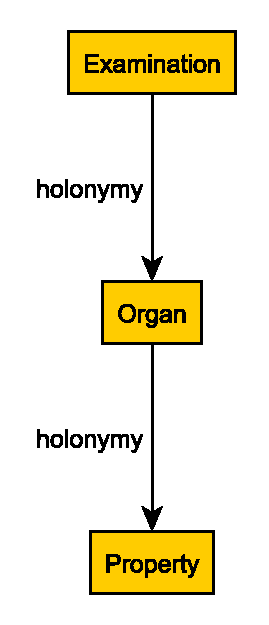
\includegraphics{report-semantic.pdf}
    \caption{Simple ontology representing entities and relationships between them encoded in reports generated using the proposed system
    \label{fig:report-semantic}}
\end{figure}

\begin{figure}
    \centering
    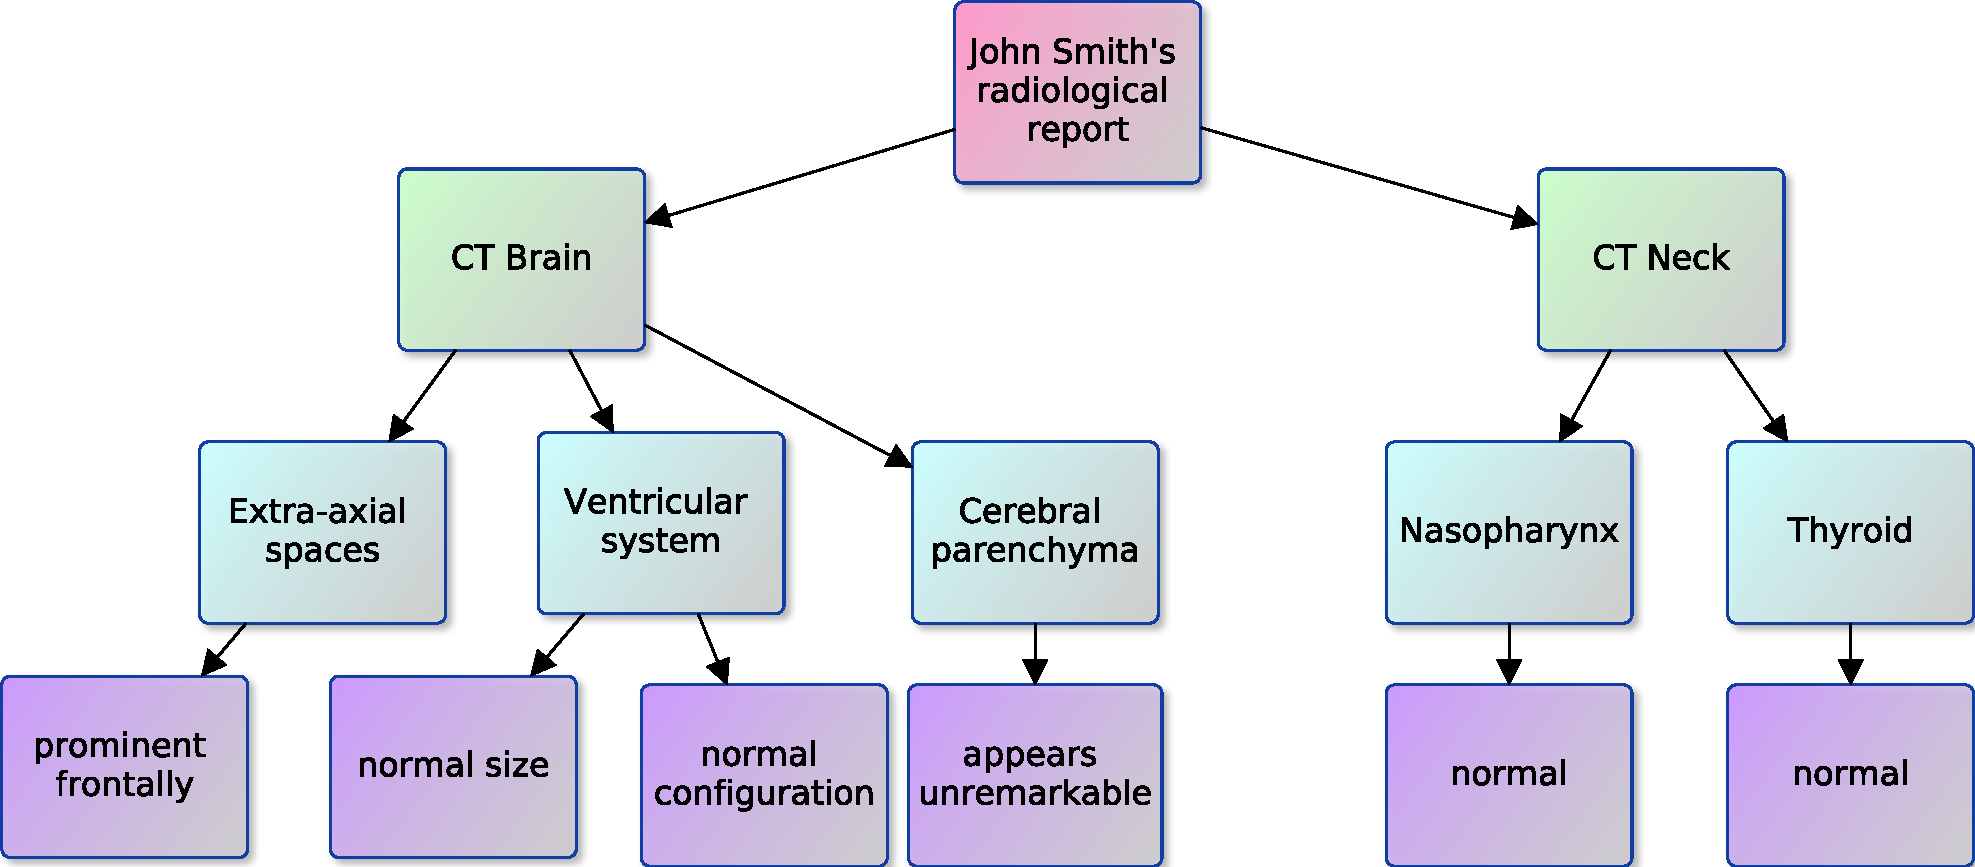
\includegraphics[width=\linewidth]{report-tree.pdf}
    \caption{Typical structure of a radiological report created  using the proposed system\protect\footnotemark} 
    \label{fig:report-tree}
\end{figure}
\footnotetext{For simplicity, only names of nodes are presented (associated meta-data were omitted)}

By using this ontology, a radiologist can create a report that is similar in structure to a tree (as it is presented in figure \ref{fig:report-tree}). At any given moment, the doctor modifies the tree at a single level, which allows for suggesting what are the items that can be included. The idea was taken from statically typed languages which, thanks to their strictness, allow for coding with smaller number of mistakes at the lexical level \cite{static-lang}.

\section{Work-flow of a radiologist who uses the proposed system}
In figure \ref{fig:report-workflow} a typical work-flow of a radiologist is represented in the form of a flowchart. 
\begin{figure}
	\centering
	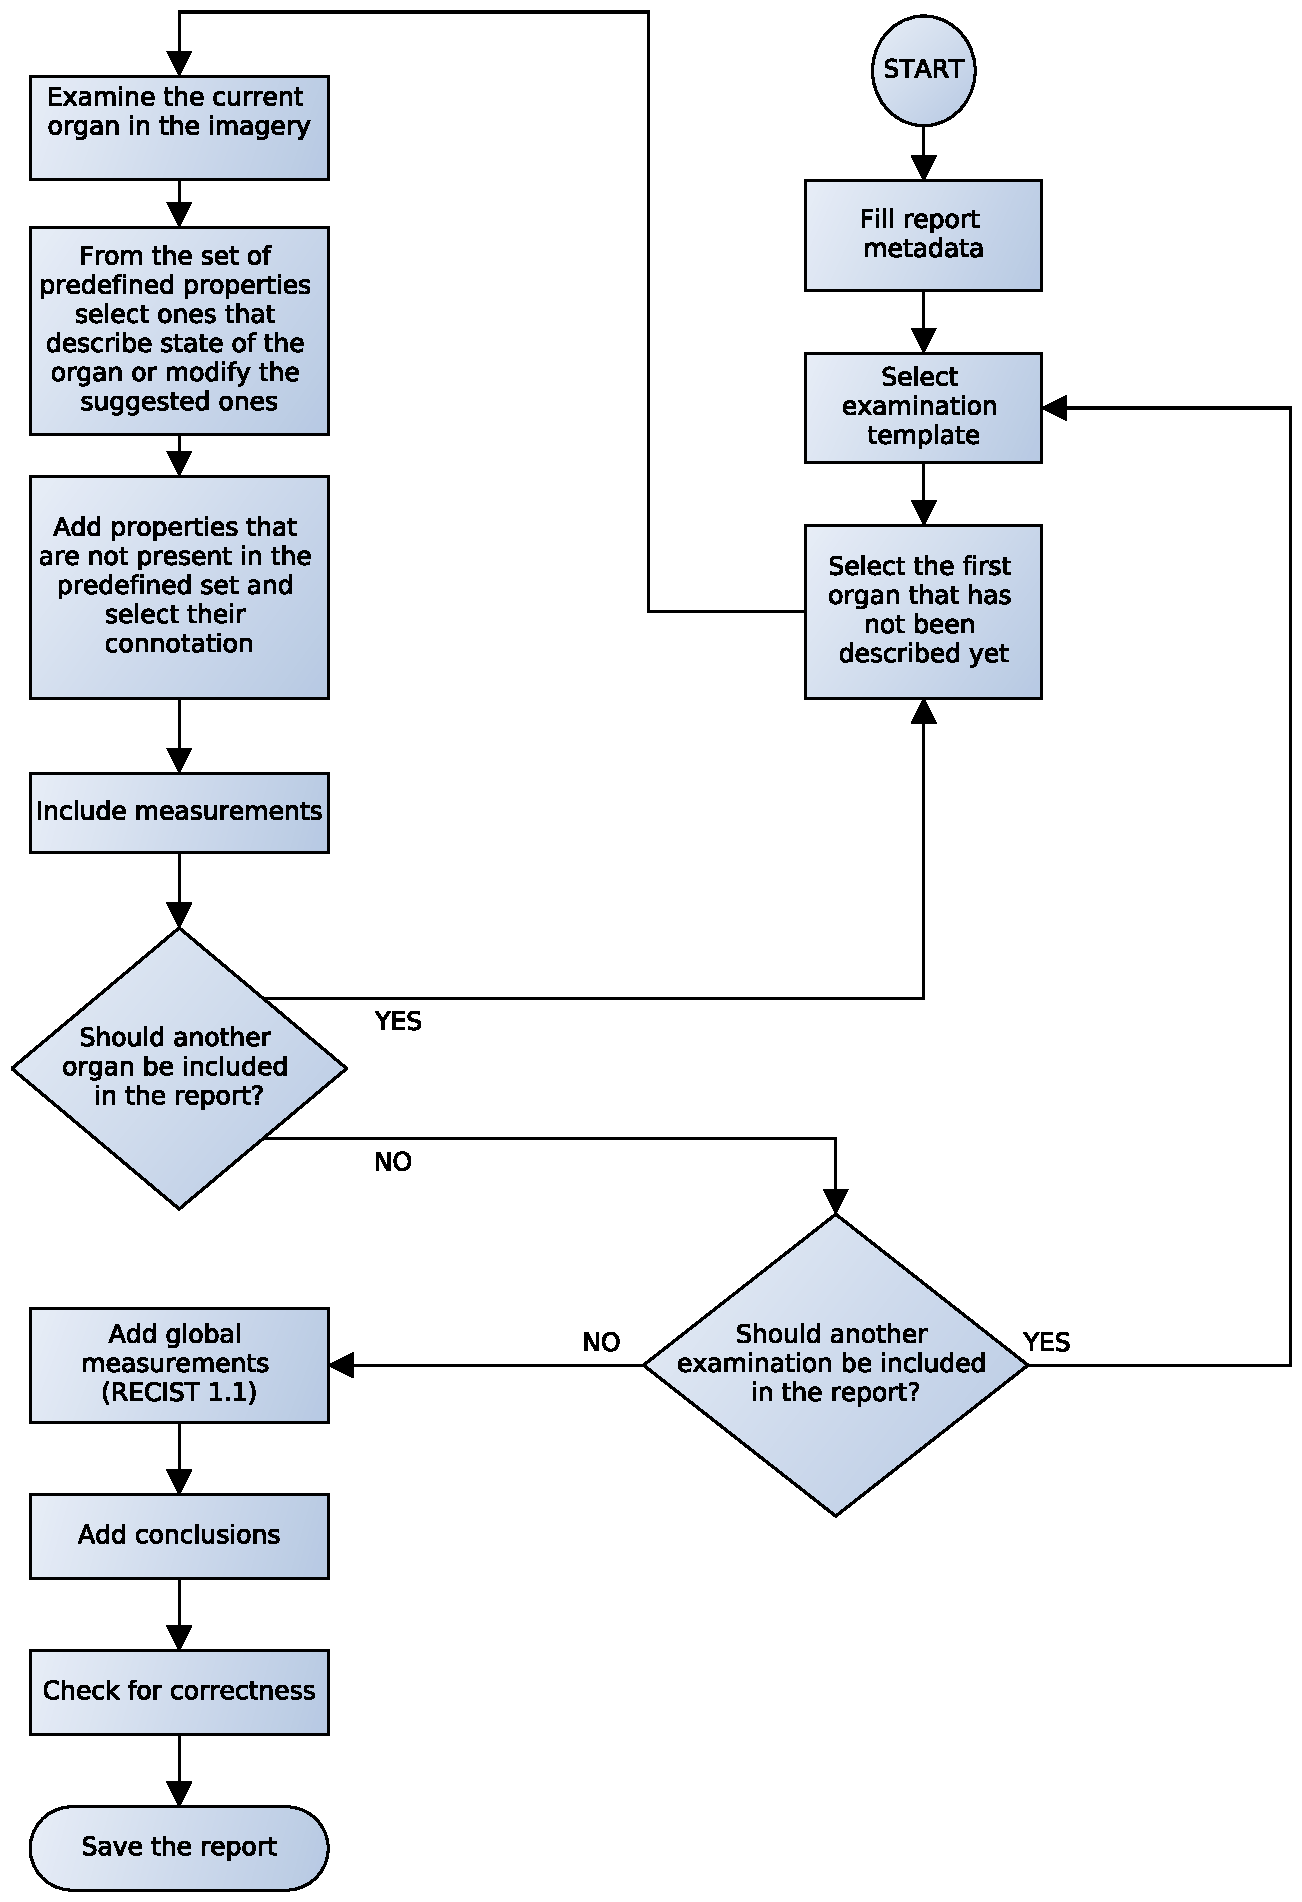
\includegraphics[width=\linewidth]{report-workflow.pdf}
	\caption{Work-flow of a radiologist who uses the proposed system to create contents of a radiological report
		\label{fig:report-workflow}
	}
\end{figure}

\subsection{Connotation}
Besides having text, each property can have a semantical attribute called connotation. Connotation is used to highlight the impact of this property on the result of the organ and examination. This attribute can have one of three values: positive, negative and neutral. Figure \ref{fig:property-connotation} presents connotation selection box that is present next to the property text editor.
\begin{figure}
	\centering
	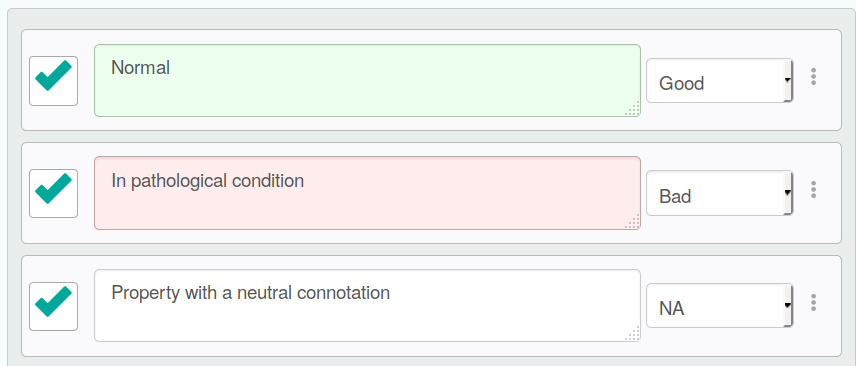
\includegraphics[width=0.8\linewidth]{property-connotation}
	\caption{Connotation can have one of three values: positive, negative and neutral
		\label{fig:property-connotation}
	}
\end{figure}

\subsection{Meta-data}
Report may also contain some meta-data which can be used to identify the patient whose body is described in it. Shape of these pieces of information strongly depends on the RIS system used in a clinic. Text segments present in meta-data have no special influence on the semantics of report so it has no detailed description in this work. Figure \ref{fig:report-metadata} presents user interface used to input commonly used meta-data.
\begin{figure}
	\centering
	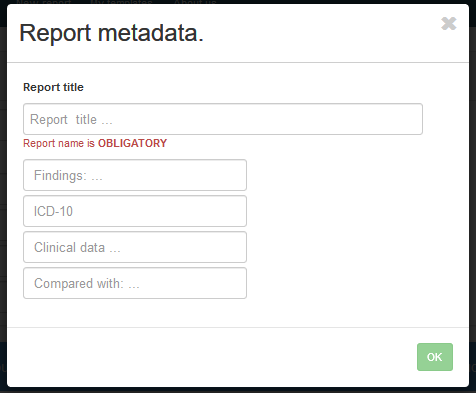
\includegraphics[width=0.6\linewidth]{report-metadata}
	\caption{Report meta-data allow user to specify general information about new report
    \label{fig:report-metadata}
	}
\end{figure}

Names for ontological structures shown in Figure \ref{fig:report-semantic} were chosen so it is easier for radiologists to imagine what they describe, however, they can be used not strictly (e.g. in a CT scan it is possible that a radiologist adds an organ that contains details about intracranial hemorrhage which is a kind of bleeding within the skull \cite{ich} but not an organ in its very meaning). This is one of the known weak-points of the proposed ontology.

\section{Examination template}
Examination template (or simply a 'template') consists of an ordered list of all organs that could be described when creating a report. It also has some portion of meta-data used for filtering like category, discipline. Templates use the same ontology as the reports as templates can be imagined as reports with all properties, organs included. 

\begin{figure}
    \centering
    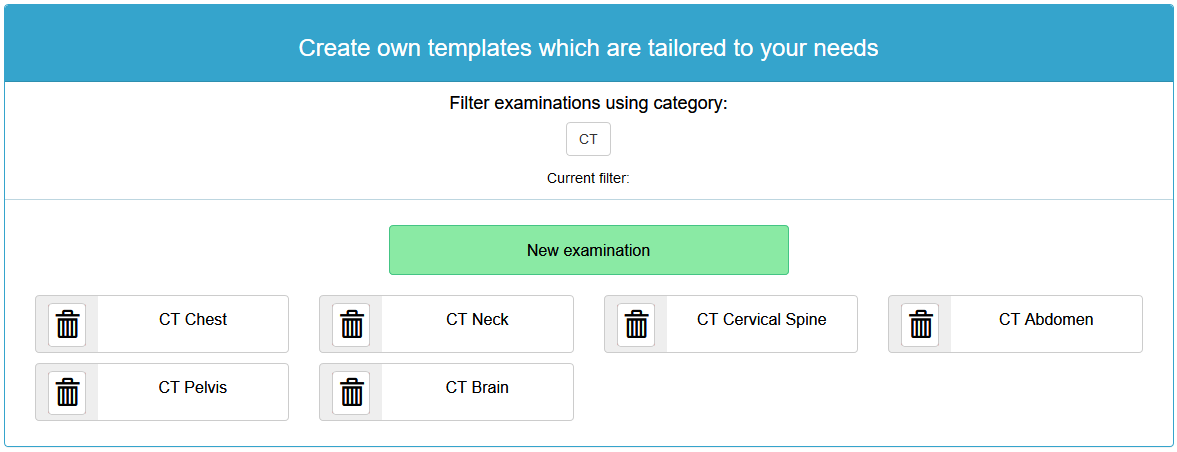
\includegraphics[width=0.9\linewidth]{templates-list}
    \caption{List of templates that can be edited by the user\label{fig:templates-list}}
\end{figure}
\begin{figure}
    \centering
    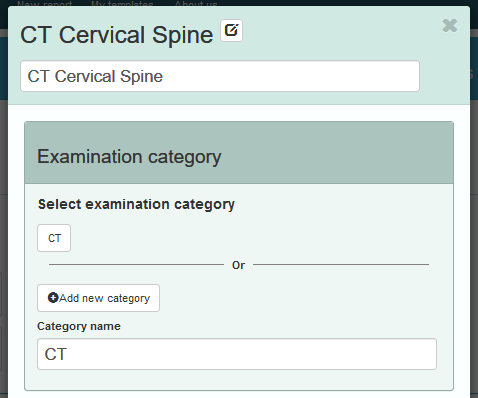
\includegraphics{template-metadata}
    \caption{GUI used to edit template meta-data \label{fig:template-metadata}}
\end{figure}
\begin{figure}
    \centering
    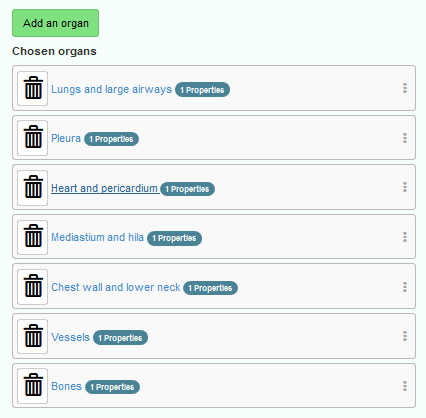
\includegraphics{template-organs-list}
    \caption{GUI used to edit organs \label{fig:template-organs-list}}
\end{figure}
\begin{figure}
    \centering
    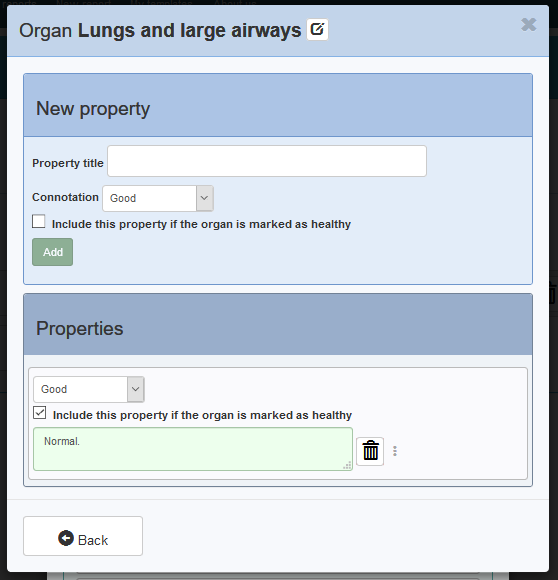
\includegraphics{template-property-list}
    \caption{GUI used to edit properties of an organ. User can predefine connotation and tell the program that this property can be automatically included if the organ is marked as healthy \label{fig:template-property-list}}
\end{figure}

Examination templates can be prepared by the leader of radiologists team, so the team can use common language to describe diagnostic imagery. Templates prepared by the leader constitute the so called set of public examinations.

If a given template is not sufficient for a particular radiologist, they can create their own template from scratch or extend the existing one (an action that for people familiar with git version control system can resemble forking a repo \cite{forking}).


\section{Productivity improvements}
\subsection{Using templates}
The goal to increase productivity of a radiologist is achieved mostly by decreasing the average time a doctor types on keyboard. Thanks to the usage of examination templates, the time spent to create the schema of the report is shifted from the doctor to the leader of the radiologists team. It can take a lot of time to create a template that is both universal and correct but it is a one-time-only investment. The more templates are created using a template, the more it pays off in the long run.

\subsection{Mark organ as healthy}
In the proposed system, each property has additional attribute (it can be set in template editor) named "include if organ healthy". When a radiologist creates a report, an organ can be marked as healthy, which means that all properties that have this attribute set to true are automatically included in the report. This allows to quickly add properties that are very commonly used. 
In order to minimize the possibility of inclusion a property that does not correspond to the actual state of patient's body, only properties with positive connotation can have this attribute set. 

\subsection{Calculators}
There exist many standardized numerical methods used to asses whether values of certain parameters are in the range suggesting poor health condition, e.g. one of the most popular parameter is the body-mass-index (BMI) which is calculated using formula:
\begin{equation}
BMI=\frac{mass}{height^2}
\end{equation} 
After calculating this index, a doctor has to look through tables to check whether the value is usually attached to people with obesity or not. 
BMI is only one formula out of hundreds of techniques used by doctors. It is not integrated, however, into the proposed system as it was decided that it is not used frequently by end-users.

\subsubsection{RECIST 1.1}
During the design of the proposed systems several radiologists who specialize in oncological medicine reporting suggested that a method called  Response Evaluation Criteria In Solid Tumors (RECIST 1.1) is of special importance to them. This method is used to assess whether tumors in cancer patients improve, stay the same, or worsen during treatment \cite{wiki-recist}. As there are hundreds of similar methods used by radiologists, it would be impossible to implement them in the proposed system all at once, so it was decided to use RECIST 1.1 as a proof of the concept of calculators that can be used in structured reports.
A radiologist, while creating a report, can measure size of lesions and write down the results of measurement in the report. Proposed program should recognize that the numerical value represents a measurement (as shown in figure \ref{fig:recist-parsing}) and should suggest whether it should be included in the calculation of RECIST 1.1 or not (as shown in figure \ref{fig:recist-config}).

\begin{figure}
	\centering
	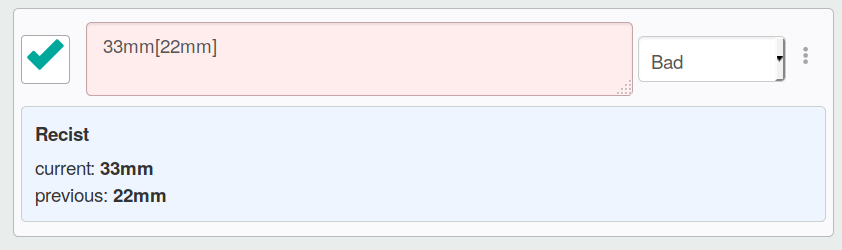
\includegraphics[width=0.8\linewidth]{recist-parsing}
	\caption{Measurements data are automatically parsed when user types text into the property textbox
		\label{fig:recist-parsing}
	}
\end{figure}

\begin{figure}
	\centering
	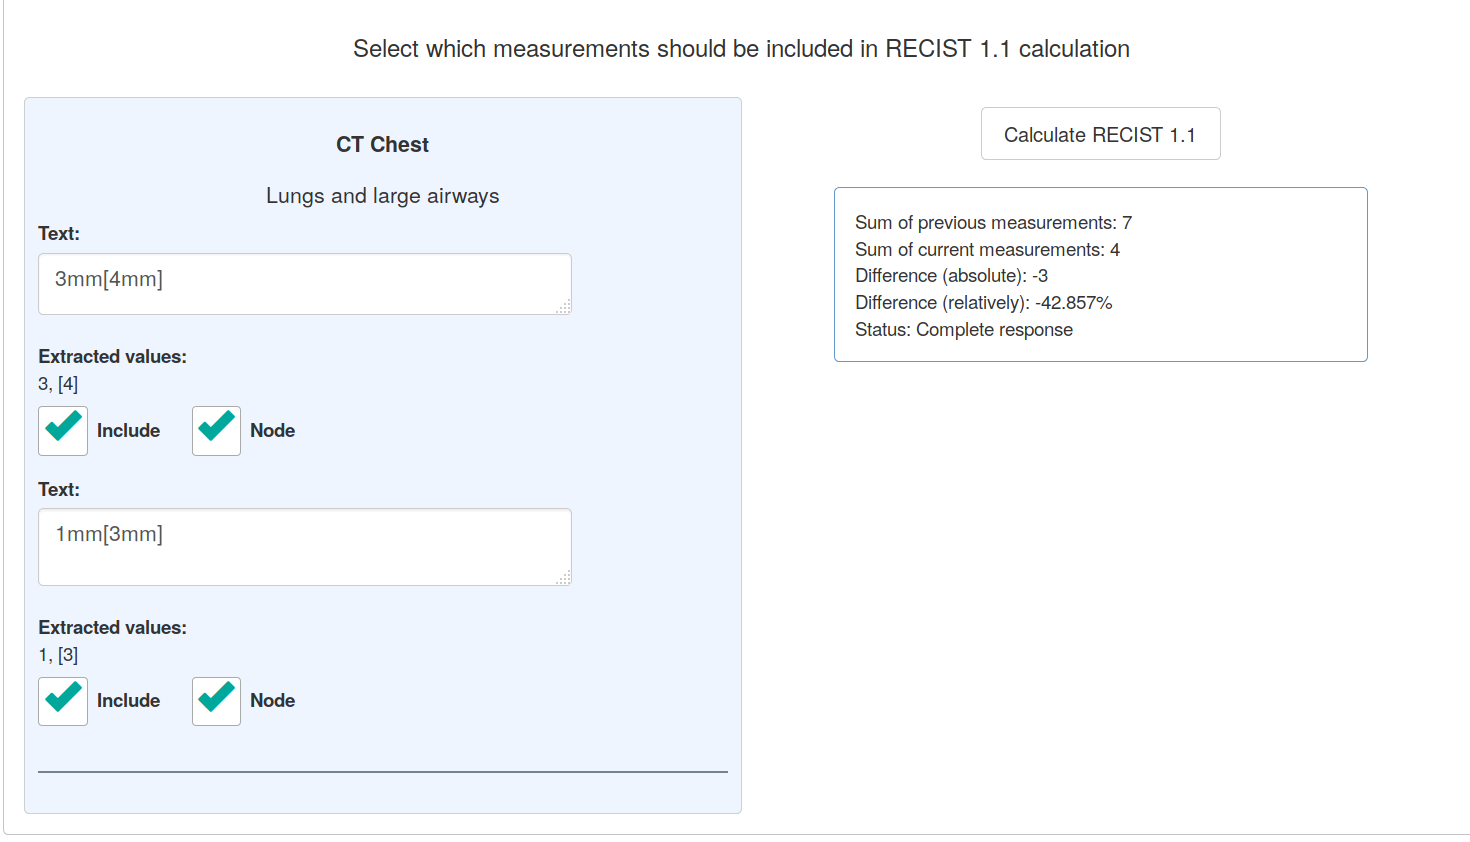
\includegraphics[width=\linewidth]{recist-config}
	\caption{Just before confirming the completeness of the report the user is asked to decide which measurements should be included into RECIST 1.1 calculation\protect\footnotemark
		\label{fig:recist-config}}
\footnotetext{There is a limit of 5 values defined in the algorithm specification.}
\end{figure}


\section{Reporting quality improvements}
\subsection{Standardized nomenclature}
There exist several attempts to standardize the language doctors use to describe precisely medical imagery. Templates created for the proposed structured reporting system can be created with the help of terminologists who specialize in systematized nomenclatures like SNOMED and LOINC to create reports what can lead to improved reporting quality as a radiologist does not have to explore huge volumes of precise textual definitions of terms used. 
\subsection{No repetitions}
Templates can be interpreted as TODO-lists containing tasks which have to be done while describing medical imagery, so a radiologist can be sure that nothing was omitted or no item appears twice in the report as a result of a mistake.
\subsection{Reports have ordered list of elements}
Reports created using the proposed system can be represented as trees, nested lists of items, so it is easy to spot relationships between properties and organs and also differences between two reports describing one patient.
\subsection{Highlighting the most important pieces of information}
The most important pieces of information can be highlighted using proper value of connotation. When one of properties of an organ should be interpreted as a main cause of health problems it is marked as a pathology. When the report is then rendered as a document, this property can have e.g. different font color, some text-decoration element or different background color (Figure \ref{property-connotation-rendered}).

\begin{figure}
	\centering
	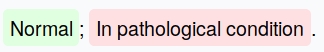
\includegraphics[width=0.3\linewidth]{property-connotation-rendered}
	\caption{Exemplary representation of connotation in the rendered version of the report: positive connotation is represented as green background of the text, negative --- red, neutral --- transparent.
		\label{property-connotation-rendered}
	}
\end{figure}
\subsection{Shift from difference reporting to the current state reporting}
There exist practices quite popular among radiologists mostly from smaller clinics that are considered as bad among professionals. One is to include in the radiological report only properties of body which they consider as bad for patient's health. Due to the subjective nature of the report there were cases when a radiologist skipped a finding that was important stating the patient was healthy leading to more difficult and expensive treatment later.
There were also cases when a radiologist was unable to compare current state with descriptions of several images that were taken at different times, only with the last one. The doctor stated that there is a progress in treatment, but in comparison to the second from the last description, the health condition worsened. \cite{risk-management}
Templates created using the proposed system can favor radiological reports that are more self-contained, it means they describe both bad and good (with respect to connotation) properties of patient's state.

\subsection{Update of the report}
Having a previous report, a radiologist can create another one that will be an update to the former. This procedure is often applied during chemotherapy to see whether tumors react to the treatment. A software functionality that allows the radiologist to introduce small changes to the report without rewriting it, would increase the quality of reporting as the resulting report would be still self-contained. 

 



\chapter{Implementation}
The proposed system was implemented as a web application. It is split into two parts: front-end and back-end.  
\section{Technological stack}

\subsection{Back-end}
\subsubsection{C\#}
As a main technology that is used to structurize data that is displayed to the user or received from them, ASP.NET C\# framework was used.
C\# is an imperative, strongly-typed, object-oriented language that is used on the market to create enterprise software. There is a hight availability of good quality tooling that makes development in this language faster and less error-prone.

\subsubsection{ASP.NET}
The ASP.NET application is created using MVC pattern (Model-View-Controller) that is widely known for helping to create applications that consists of loosely coupled, pluggable components. Some interactions with user interface result in HTTP requests that are then mapped by the server to routes that are forwarded to Controllers. Controllers are used to react to user action, instantiate proper classes which implement application logic (they are part of the Model), feed them with sanitized and validated user input and invoke proper methods. When the results of execution are present, Controller finds a View that is expected to be used to present results to the user. View can be treated as a template for the data that is returned from Controller. It can be an ordinary HTML file with placeholders for certain pieces of information (it can also include formatting) or even JSON or XML documents that are only concerned with shape of the data, not the visual representation (e.g. formatting).

\subsubsection{Entity Framework}
Entity Framework is a set of libraries that is used to create high-level abstract model using C\# that are then converted to sets of relations and attributes in the underlying DBMS. It can also be used to transform LINQ constructions to SQL queries taking into the account vendor-specific features of many DBMS.
The approach of first creating C\# classes that represent Model and then automatically converting it to the database relations and attributes (scaffolding) is called Code First Approach. It can be especially useful when the schema of database changes very often. When changes are introduced to the code representing Model, Entity Framework can be used create a migration  -- set of transformations for DB schema that after applying to the DB will keep code and schema synchronized. 

\subsection{Database}
MSSQl server is used as a DBMS because it is a battle-tested, well-documented solution that can be easily paired with ASP.NET and Entity Framework's code generation methods are best optimized for this particular DBMS. 

\subsection{Front-end}
Not all interactions with the application result in HTTP requests sent to the server, many of them are about shaping data that has already been received from the server. In order to make use of this fact main part of the application -- tabs: New Report and Templates were developed as a Single Page Applications (SPA) in order to minimize the time that user has to wait between actions they take. Technologies used in these parts are JavaScript and AngularJS framework. 

\subsubsection{JavaScript}
It is a very popular scripting language that can be executed in any popular web browser. Version of the language used in this project is ECMAScript 5.1 compliant. 
\subsubsection{AngularJS}
AngularJS is a JavaScript framework that helps with building MVC SPA aplications. It has several mechanisms like two-way-binding that reduce size of the code needed to implement Create, Read, Update, Delete (CRUD) functionality.


\subsubsection{Razor views}
The remaining front-end subpages are generated using view engine present in ASP.NET called Razor. These views are responsible for interactions like logging in , registration (backed with ASP.NET identity mechanism), listing reports, searching for particular report etc. They are generated on the server side and sent to the user as HTML and rendered by the browser.
 


\section{Internationalization and localization}
The application was designed to be accessible by radiologists from many countries, so support for many languages is one of its core functionalities. The application automatically detects user preferred language by looking into user browser settings. Each of the most popular Internet browsers allows users to specify list of preferred languages used by web-pages. The presented solution scans this list and chooses first language it supports, if there are no languages in the list that are supported, English language is presented to the user by default. Figure \ref{fig:language-preferences} shows how this list can be manipulated in one of most popular web browsers.
\begin{figure}
    \centering
    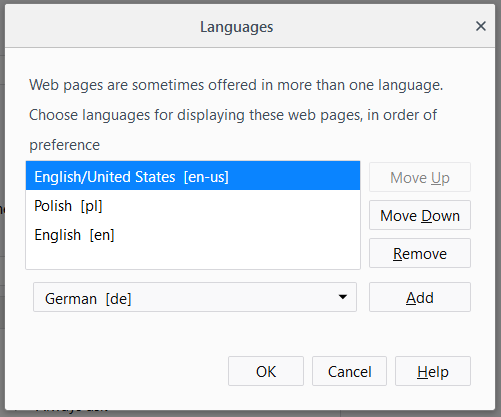
\includegraphics[width=0.6\linewidth]{language-preferences}
    \caption{Language preferences list present in Firefox 54\label{fig:language-preferences}}
\end{figure}

At the back-end there are dictionaries for each supported languages that contain mapping $name \to value$. 
In Razor views names are used to specify where particular piece of text should be placed. During HTML generation, the application resolves user language and refers to proper resource file. Figure \ref{fig:language-dictionary} presents contents of a dictionary for ReportWizard for Polish language. Adding support for another language is simply providing values for existing names in the dictionary.

For SPA parts of the program the situation is slightly different as DOM elements representing most of their content are generated at the user side with the help of AngularJS. In order to have single source of truth about translations, it was decided to serialize contents of dictionaries to JSON format, and send it to the user with page template. At the front-end the translation dictionary entries are deserialized and made available to JavaScript functions. This solution makes it faster to edit and version translations as they are kept in a single place. One of drawbacks can be the performance of this solution, but it was measured that for number of dictionary entries used in this application, the decrease in performance is negligible.
 
\begin{figure}
    \centering
    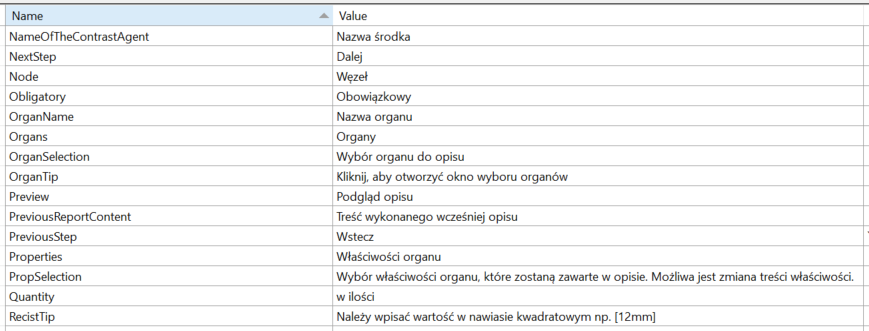
\includegraphics[width=1\linewidth]{language-dictionary}
    \caption{Dictionary for Report creator for Polish language\label{fig:language-dictionary}}
\end{figure}
\section{Templates}
Templates can be manipulated by the user at the examination level. Users can create them, edit, remove. In order to keep things simple and less error-prone, they are treated as immutable in the database. If user edits a template, the previous version of the template is deleted and template version with edits is inserted into database. The only thing that is not changed in this process is its primary key. This makes reasoning about database queries much easier and has satisfactory performance for templates used by most radiologists. Thanks to the use of database transactions, one can be sure that removing contents of an existing template and inserting contents of a template with modifications is performed atomically.

\subsection{Feeding front-end with data from database}\label{templates-immutable}
After browser finishes loading static files (scripts, fonts, etc.), an additional HTTP request is created to download report templates attached to the current account. Server handles the request by querying database, instantiating model classes that correspond to the data received from database. Finally, server serializes reports data to the JSON format and sends it to the front-end. When front-end receives JSON data, a success callback is invoked and sets the data as current view model. 
From now on a user can edit any existing template: add properties, organs, remove them, change connotations, reorder elements. Thanks to the two-way-binding mechanism, user interface can be directly connected with references to the fields of an object so the developer can focus on the visual representation of the editor. In order to make editor more robust, length of text contained in it is measured on each onChange event and its height is adjusted, so all its contents are visible to the user.
\subsection{New Examination}
User can create new template by clicking on New examination button. Then they are asked to input title of new examination. One of requested features was the ability to copy contents of existing examinations what is similar to forking in git. In order to achieve this, when modal window with new examination's title is opened, front-end loads from server list of user-owned examinations concatenated with list of publicly-available examinations. The latter allows users to quickly customize templates prepared by the administrator.

\subsection{Edit examinations}
On page load all templates that are owned by the user are downloaded. Any modification can be applied: renaming, reordering of elements, setting connotation, etc. When user clicks Save button, actions related to the immutability of templates described in section \ref{templates-immutable} are performed.


\section{Report creator}

\subsection{Data loaded lazily}
Report creator is the most optimized part of the application. It is the place where user spends most of their time and it has to respond to any action immediately. It is not easy to predict which examinations will be used in a particular report, so all of available examinations must be ready to be loaded. At the page load, only list of available examinations' titles (user-owned and public examinations) is loaded from the server. When the user clicks on examination's title, the rest of template's content is loaded via HTTP call and ready to be modified and included in the report. Figure \ref{fig:examination-list} shows the initial screen of a template editor with titles of templates listed.
\footnotetext{Initially only a list of names of available templates is presented to the user. Contents of the template are downloaded after clicking on the pill representing a template}
\begin{figure}
	\centering
	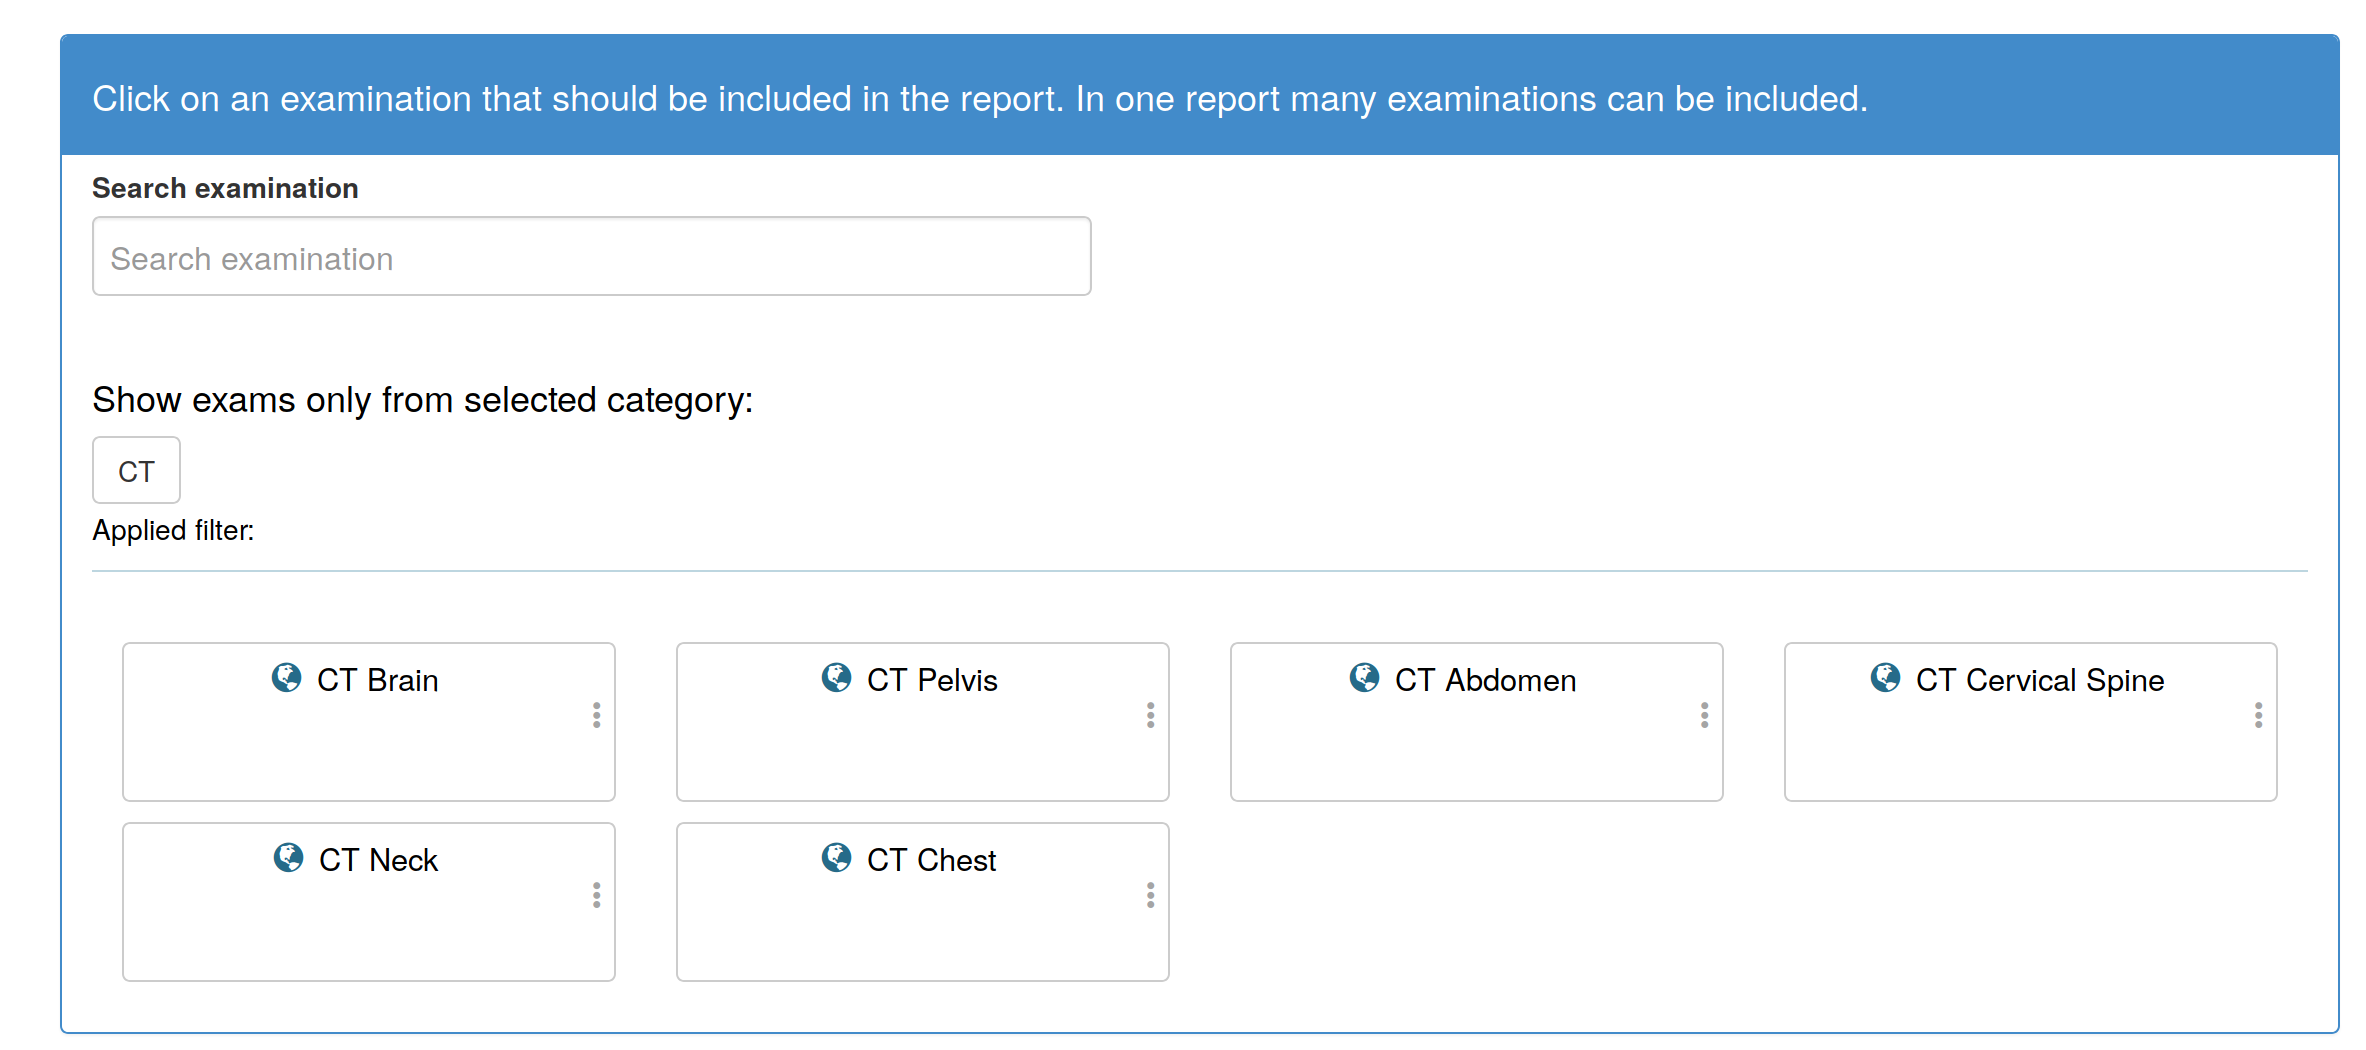
\includegraphics[width=\linewidth]{examination-list}
	\caption{A window demonstrating list of examinations to the user\protect\footnotemark
		\label{fig:examination-list}
	}
\end{figure}



\subsection{Caching at the user side}
When radiologists are specialized in a particular field, they have subset of examinations that they describe most often. Loading examination templates separately each time they create a report, would be a waste of time. In order to solve this issue, a caching mechanism at the user side was designed. After loading, JSON data describing examination elements are saved to the storage managed by the browser called localStorage. It is a dictionary-like storage that can be used from JavaScript to save string values. When user tries to open an examination, the localStorage cache is checked whether this examination is present. If the examination is in the cache, it is immediately shown to the user. Otherwise, an HTTP request to the API is issued to download data.

\subsubsection{Cache invalidation}
As templates contain no sensitive information, they can be stored in localStorage without restrictions regarding synchronization of cache invalidation with session expiry time. However, the invalidation has to happen when user updates an examination in the Templates tab. In order to keep things simple, the whole cache gets purged anytime user navigates to the Templates tab. 

\subsection{Editing functionality}
As user navigates through the levels of the report structure, the program signifies this by opening modals windows one on top of another. This results in the following behavior: when user makes decisions that have the biggest impact on the shape of the report -- edits report meta-data, selects examinations that will be used -- the program is at the 1 st level of depth, no modals are present.
When user decides to include an examination, a modal is opened hiding all information that is not necessary at the moment and the user is shown list of organs with preview of the report (As shown in figure \ref{fig:organ-list}).
\begin{figure}
	\centering
	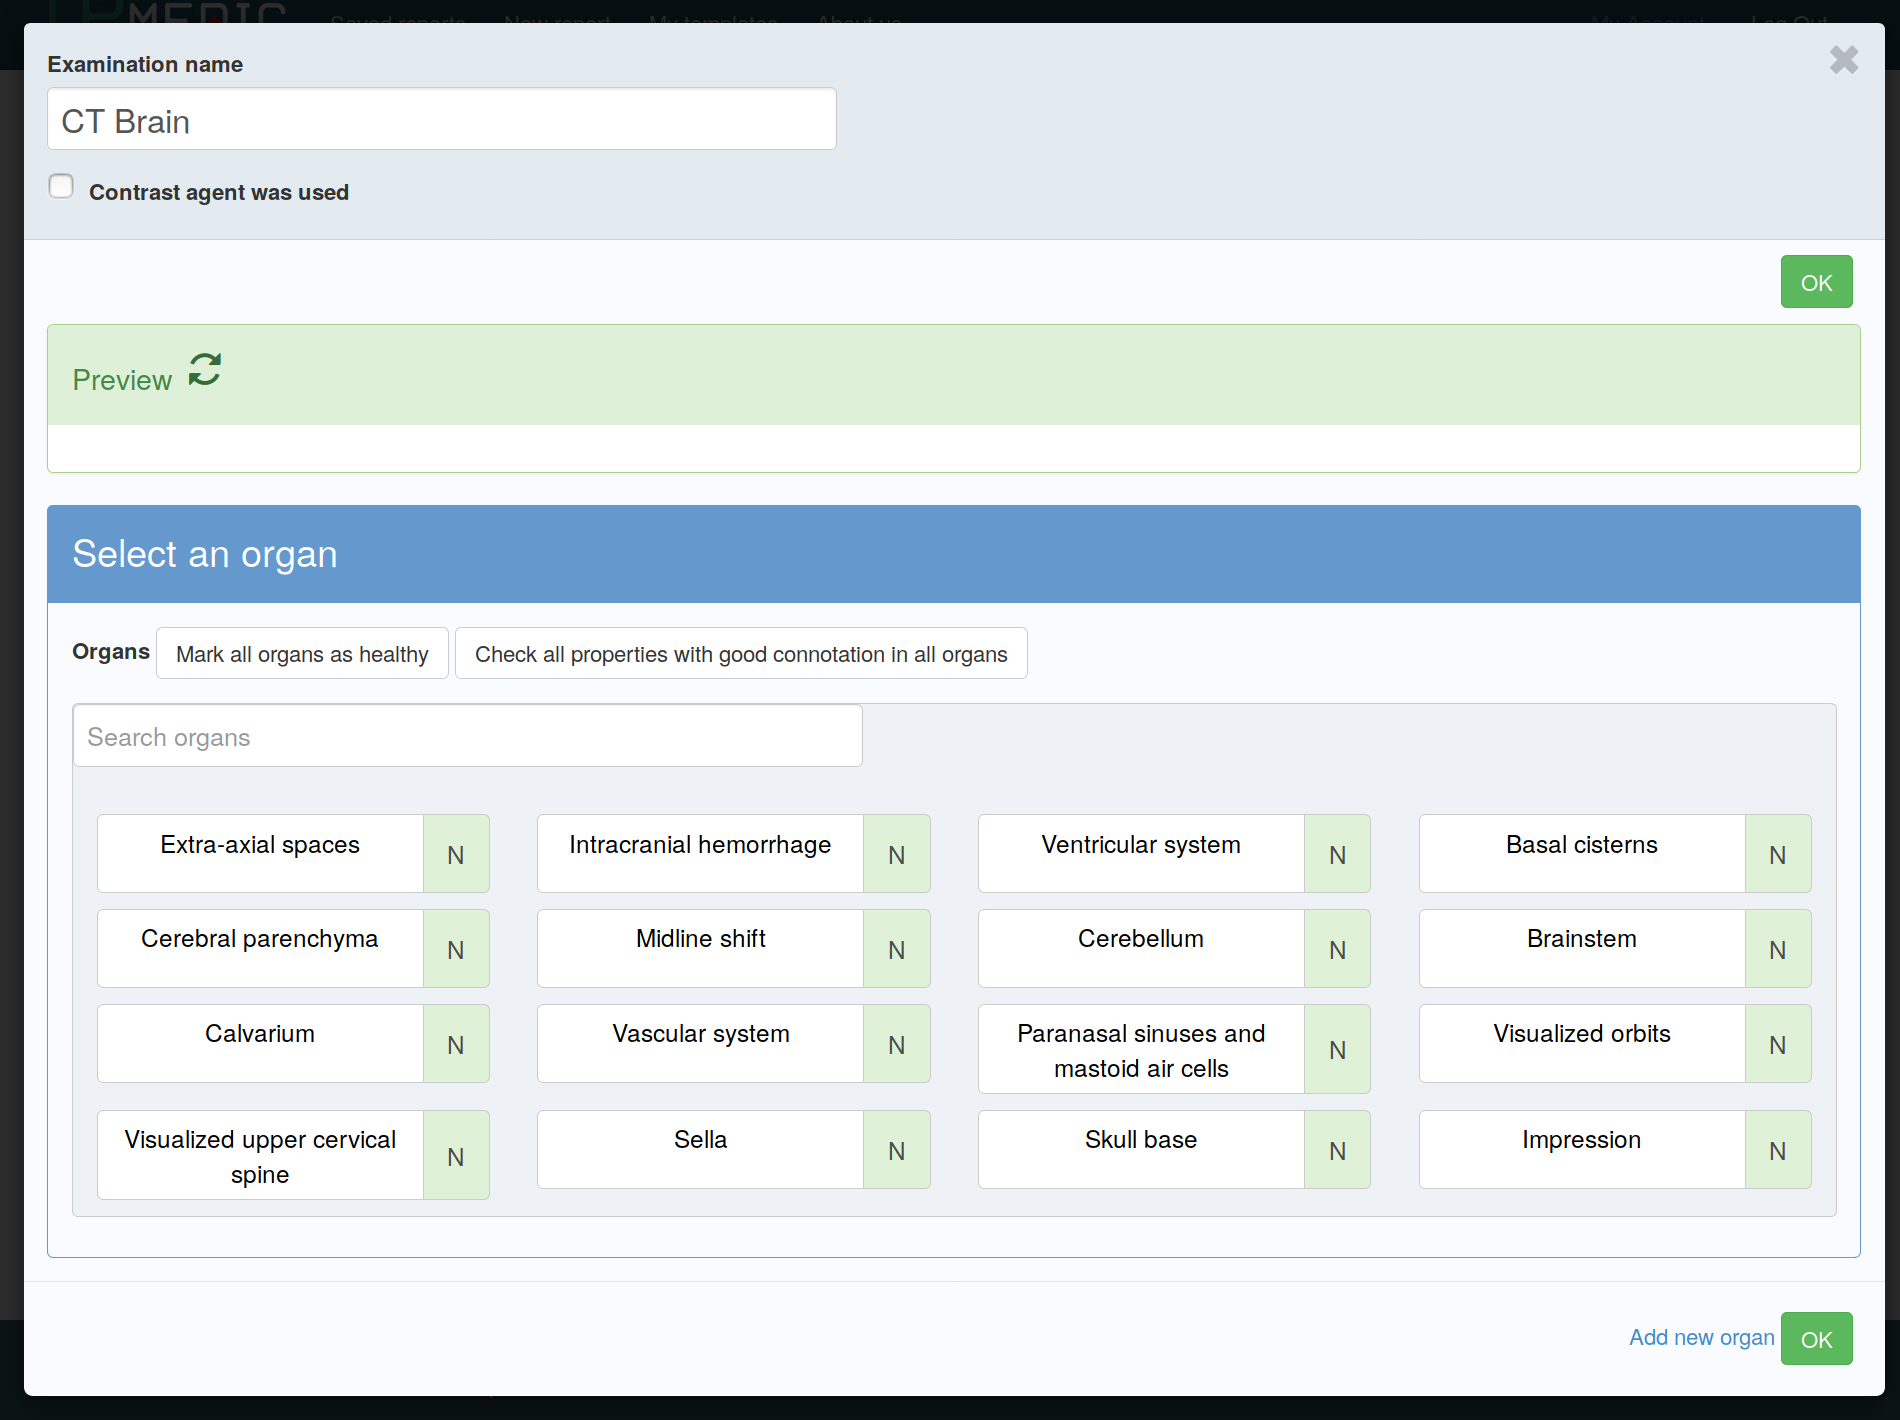
\includegraphics[width=\linewidth]{organs-modal}
	\caption{List of organs defined in a CT Brain examination template
		\label{fig:organ-list}
	}
\end{figure}
Work-flow is designed to favor selecting Examinations/Organs/Properties from predefined sets. It was measured that with suggested use of the templates on average 82\% of report's content can be generated from template contents. As most of the content can be added to the report by simply clicking on a check-boxes, a lot of thought went into designing interaction model that allows radiologists to look at sequence of suggested elements and make a binary decision 'yes' or 'no' whether an element should be included in the report or not. 
As the program can be used on any device, it can be interacted using mouse or using touch. When the program is executed on a device with mouse, the font-size and check-boxes are smaller as user uses mouse to precisely click on them. When the program is executed on a smaller device like tablet or smartphone, some elements are shrunk but check-boxes become bigger, so it is easier to tap them. 

\subsection{Predefined but modifiable}
In some situations edits must be made to the predefined pieces of text. This was solved by putting any report text in a slightly customized text-area that is attached to AngularJS context. The text-area is aware of the length of text it contains and automatically fits its height to show the whole text to the user at any time.


\subsection{Live preview}\label{live-preview}
It is crucial for the user to always be aware of the impact of edits they make to the report contents. Live preview mechanism was designed specifically to solve this. Any significant change of context or report contents sends an event to the function that filters elements that were selected and generates report's textual representation. As this function can take a lot of time to execute, it cannot be left to AngularJS to decide when it should be called (infamous \$digest cycle \cite{angular-digest}) as it would have a severe impact on performance. AngularJS internally observes arrays of data that are attached to its scope to look for changes, so it was decided to call this function only in several situations, e.g. when report-context is switched, a property is checked etc. but not on every single text-change of the report. This allows the user to have a seemingly live preview of the resulting report while focusing on selecting predefined pieces of text.
\subsection{Changes propagation}\label{changes-propagation}
Connotation it attached to each property, however, it is also useful to see its effect on the organ. This way, it is easier to see which organs are in pathological condition, which examinations contain unhealthy organs. Status of an organ is calculated by accumulating connotation of all its properties: if one or more properties have negative connotations, the whole organ is marked as in unwanted condition. On the other hand, the organ is marked as healthy if all properties have neutral or positive connotation.
The same holds for examinations, but states of all its organs are taken into account. Propagation of the effects of connotation is done when an organ is closed. Then the accumulated connotation is calculated at the organ and examination level.

\subsection{Storing a report in the database}
This is a very important decision from the architectural perspective. Format of the saved report can impact the performance of retrieving saved report, interoperability with other systems, etc. The format of stored report could be a topic for a very broad discussion. In order to maintain the simplicity of the whole project, it was decided to store JSON representing the report in the database. Many of the DMBS have special functionalities that are based on ideas used in NoSQL databases, especially document databases to allow for storing JSON objects, validating and querying them as if they ware part of the relational data. This makes it easy to store data that can have numerous optional fields. Unfortunately, MSSQL Server does not support storing JSON objects natively (Microsoft calls their limited way of supporting this format as \textit{built-in JSON support}\cite{microsoft-json-support}), however, it is possible to store JSON string representation in a column of type NVARCHAR and then validate it on SQL INSERT by the use of ISJSON function.

\section{Report history}
Report history is a part of the program that is used to list saved reports, search for particular ones, request pdf version of reports, sending report content via email. Users can invoke on existing reports such important actions as editing them, deleting them, comparing them. As one user may have created thousands of reports using this program, this part of the program paginates reports. There are 10 reports per page and user can increment index of the page they are currently viewing or decrement it. 
One useful feature is grouping reports by title. This is useful when user has the convention of naming that report's title is always name of the patient (most of the current users of the program do it in this way) as they can see and count reports for any user organized in groups. 

\section{Compare reports}
This feature strongly depends on the mechanisms included in the Report creator. It copies meta-data of an existing report and creates a new report using it. Content of the old report is presented to the radiologist as a reference and it is also copied as a basis of a new report. When the doctor makes some changes to the contents of the report, only the new version is modified. This allows for fast creation of a report that has only small portion of fragments modified when compared to the previous one.
TODO: describe changes propagation

Figure \ref{fig:compare-report} presents interface that makes if easier for the radiologist to compare two reports.



\begin{figure}
	\centering
	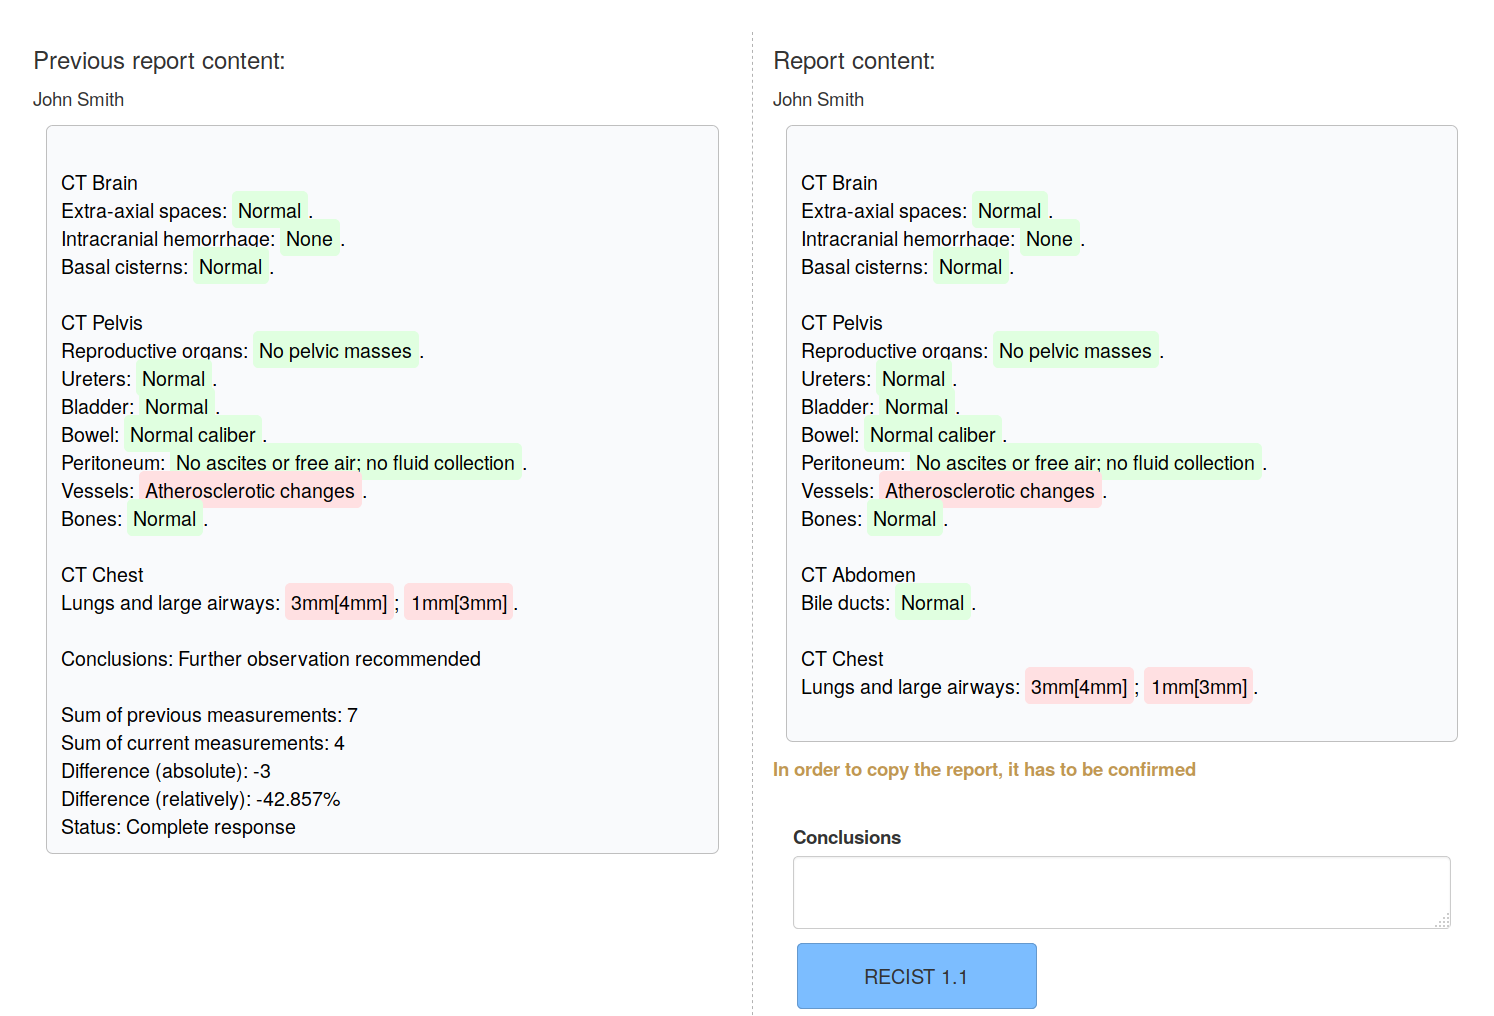
\includegraphics[width=\linewidth]{compare-reports}
	\caption{Compare reports mode presents simultaneously contents of the currently edited report and the old one
		\label{fig:compare-report}
	}
\end{figure}

\section{Integration with existing systems}
As there are many ways to store radiological reports. Many radiologists work remotely for several companies that have different RIS systems. From the practical point of view, it is very difficult to integrate the system with all of the systems as it often requires cooperation of both developer of the proposed system and the developers of the RIS system. 

Current approach to integration is very robust, works for all of the systems used nowadays but is not very elegant from the point of view of software engineering. 
After generating the report using the proposed system, it is the radiologist's duty to manually copy the resulting report to the RIS system. It is simplified in a way that the report is automatically copied to the clipboard after clicking on its content.

On the other hand, the proposed system was designed in a way that, at least theoretically, makes it easy to create communication channels that can be used to integrate this system with existing RIS systems. This could be achieved by using Razor templating to generate messages that would be HL7-compliant. 

\section{Utility modules}
The system was designed as a solution that could be used remotely without personal help of the creator. Because of this, several modules that would make it easier to start working with the program were implemented. 
\subsection{Technical support module}
This part of the program is used to communicate between radiologists and people responsible for correct operation of the system. 

\section{Deployment strategy}

Figure \ref{fig:continuous-deployment} presents the sequence of actions and set of subjects that are required to deploy the application.
\begin{figure}
	\centering
	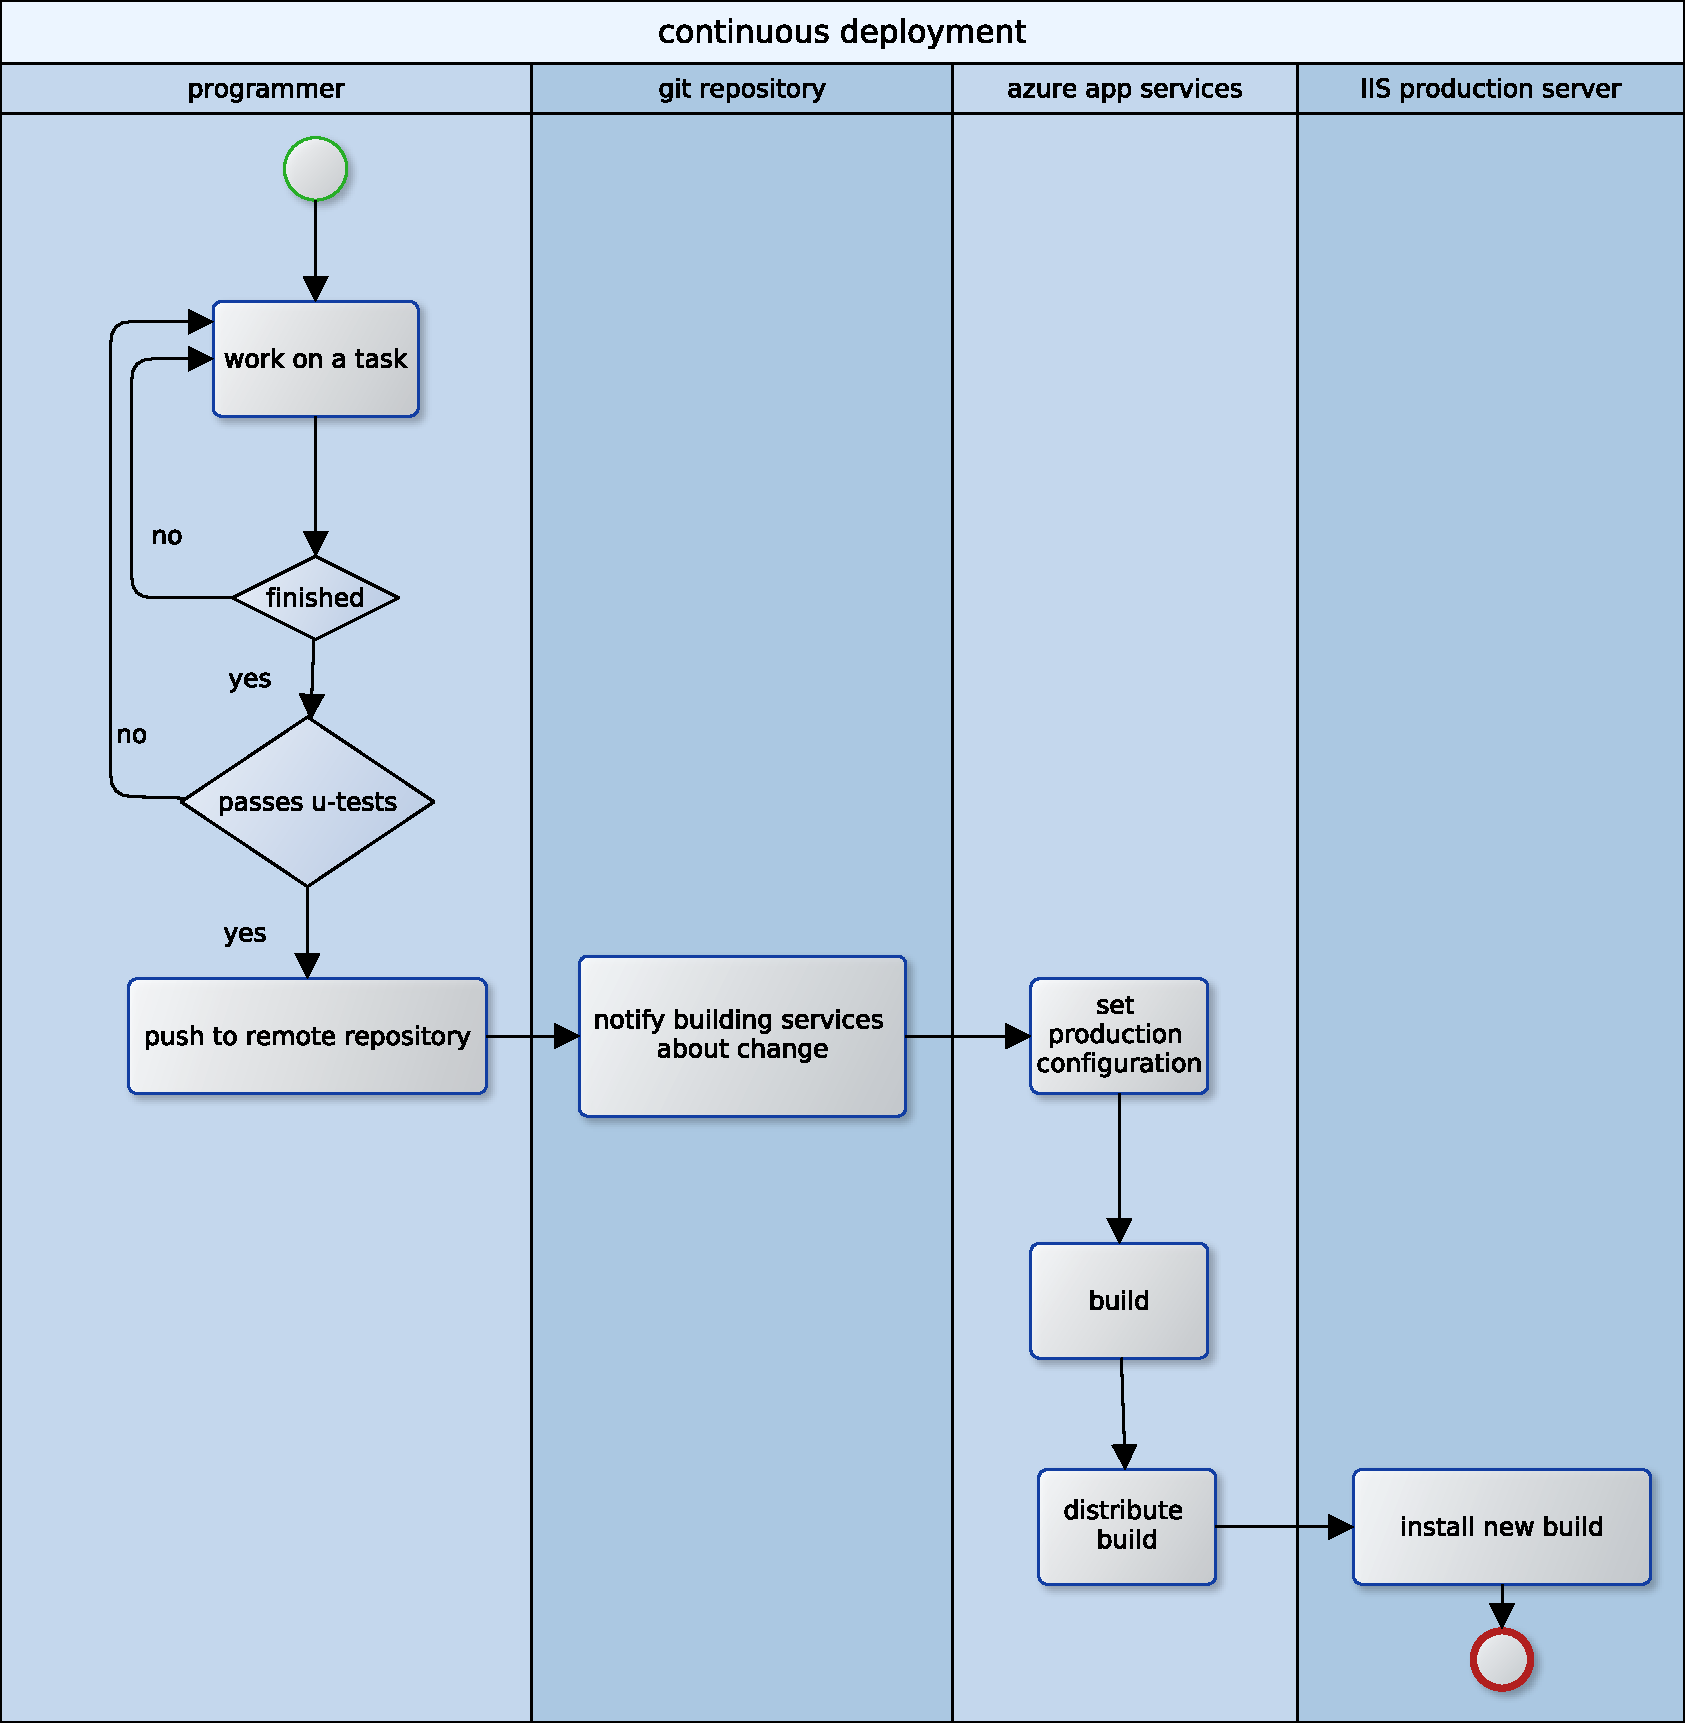
\includegraphics[width=\linewidth]{continuous-deployment}
	\caption{Continuous deployment setup makes it faster to distribute new builds to the production servers
		\label{fig:continuous-deployment}
	}
\end{figure}

\chapter{Testing and verification}
Most of the testing and verification was performed as user-acceptance testing as the program is heavily focused on interaction with user, however, security-critical parts of the program were unit-tested.
The tests were split into several classes that are described in the following sections. 

\section{Entity ownership tests}
Any piece of software that is  used to support health care requires special measures to be taken to create a product that ensures that patients' privacy is respected and no information is shown to a third party. Entity ownership tests are used in the system to verify mechanisms that filter data, so they see only data that is public or related to their patients. 

\subsection{User sees only their reports}\label{report-owner}
When user navigates to the Report history subpage, they should only see reports created by them. Moreover, manual manipulation of web browser address should also forbid accessing reports that belong to other users -- HTTP error 403 (forbidden) is thrown.
\subsection{User can edit only their reports}
Very similar to the scenario described in \ref{report-owner} but relates to the report editing functionality.

\subsection{User can access contents of public and custom templates}
When the user navigates to the ReportWizard subpage, they see a list of reports that contains both public and custom templates. They are not allowed do download other user's custom report.


\section{Database consistency tests}
Database consistency tests are used to check whether all possible mechanisms provided by DBMS are applied to ensure that related data are properly treated when an entity is removed, relationships between entities are properly split into relations, etc.

\subsection{Cascade removal}
	Deleting a user causes removal of all their reports, templates from the database. This way the system allows the user to be forgotten when it is no longer used.
	The same should hold for almost all one-to-many relations – removal of the entity that is being pointed to should result in deletion of all entities that point to is, but not the other way round!

\subsection{Code First schema generation}
	Schema of the database is automatically generated using Entity Framework Code First approach, so it requires verification whether actual schema is the same as expected. 
	Relations are created with respect to convention of naming fields of C\# classes.

\subsection{Validate JSON} \label{valid-json}
	In general, any user input should be treated as a potentially harmful. In case of reports, they are represented using JSON format. Any inserts of reports should check whether the data has all properties of a valid JSON format.
	
\section{Report structure tests}
	Thanks to tests in \ref{valid-json} it is known, that the shape of data is a valid JSON, but it not clear whether the JSON representation has all required fields, data types, etc.

	\subsection{Validate JSON representation of the report}
		In this step, JSON representation is validated whether all fields have proper names, values of fields have expected data type, types of nodes are nested as presented in the proposed ontology in \ref{proposed-ontology}.
	\subsection{Report rendering}
		The report can be easily transformed from JSON representation to HTML that can be stored in RIS systems. However, if a JSON field has content that is valid HTMl, or even worse, JavaScript script the rendered report content could be harmful to the user because it would execute unwanted code in the browser. In order to make sure, the user is not harmed while using the system, contents of all JSON fields are HTML-escaped.

\section{Report editor functionality}
	This class of tests is difficult to automate as they mostly verify user interface. All of them were performed manually as user-acceptance tests.
	\subsection{Live preview refresh rate}
	The reason for not refreshing report contents on each pressed key was described in \ref{live-preview}. These tests are performed to check, if the performance of the program is satisfactory – they are performed using a report that is considered to be unrealistically large and latency is observed. 
	\subsection{Tree changes propagation}
	Verify whether change of connotation of a property propagates into the organ and examination.
	


\section{Internationalization tests}
Currently the program has no users that do not speak Polish, so there was no special motivation to automate testing of the internationalization functionality. It was verified manually by user-acceptance tests using web browsers with different locale-settings.
\subsection{Language specific templates}
User that has the web browser language preference to English should see report templates in English, report items and meta-data entries should also be rendered in English. This should work analogically for any other language supported.




\chapter{Validation}

\section{Time savings}
The easiest way to validate the proposed productivity improvements is to measure the difference in report turnaround time. Prior to using the software, a group of radiologists was observed to measure the time it takes to create a report. The time was measured for each of the most popular examinations e.g, Abdomen Ultrasonography, Brain Computed Tomography, etc. for reports that were created using traditional methods. Then, the radiologist was allowed to use the software for several months, create their own templates. After some time for adjustments and getting accustomed to the proposed work-flow, the time to create a report was measured one again. The biggest time savings were observed for patients that were healthy or their symptoms were frequently observed. However, significant increase in productivity was also measured for reports containing unusual and complex observations. Overall, doctors who used the program with battle-tested templates and figured out what the strengths of the solution are, benefited from using the system by decreasing report turnaround time to a third of the time required to create a report without the use of the  proposed system. 

\section{User satisfaction surveys}
Over the time of first few months after the release of the software to the  users, several surveys were conducted. The users were asked open-ended questions such as: "What is the most important feature that you would like to use everyday?", "What is your overall experience you have when you are interacting with the program?", with addition to scale questions like "How likely would you recommend the software to your colleague? 1 – very unlikely, 5 – very likely", "Using the software as my main text-editing tool makes me more productive. 1 – strongly disagree, 5 – strongly agree".

It could be observed that users who initially assigned good marks to user experience, were keener to suggest further improvements. Moreover, quick reactions to the suggestions, tended to result in better marks in the subsequent surveys. On the other hand, users that were not interested in using additional tools to be more productive, were very difficult to encourage to try using the software for a longer period of time. The best results were achieved when a director of radiology observed benefits of using the program and taught their team how to use the system.


\section{Teleradiologists}
Structured reporting system is being used by several independent teleradiologists in Poland as their main text editing tool. They receive reporting requests with images they are asked to describe. They use several RIS systems from different vendors to store reports they generate. Most of them simply copy and paste reports from the system to the RIS systems they are obliged to use. As majority of the teleradiologists who have used this software are paid on the per-report basis and the average time to create a report using this program is on average three times shorter, most of the users observed significant increases in their salary. 

The system is deployed to Microsoft Azure IIS server and is globally accessible, which makes the updates easier to install and new users do not face problems with execution policies. However, it is forbidden to enter as report meta-data any piece of information that could be used to identify the user because of privacy policies in the European Union. 

\section{Hospital}
Proposed system was used in hospital in Wieliszew by a group of radiologists who specialize in oncological reporting. Reports created there were lengthy, as this specialization requires very often comparisons between many points in time to asses reaction to chemotherapy. The workflow was organized in a way that a radiologist had a group of patients they are assigned to, so it was easier to remember the treatment history of a patient. Radiologists who worked in Wieliszew provided precious feedback and many of their suggestions were included in the system. Several extensions were developed to make state comparison easier, e.g., grouping reports by title, so the radiologists can see history of a single patient easily. 
Report templates were shared between radiologists, so each new user could start getting to know the software without the tedious step of creating their own templates. Changes to templates were propagated to all users automatically, so the team could discuss what the best phrasing of symptoms are. A lot of effort has already been made to create standardized terminology by the nosologists who worked on LOINC and SNOMED, but unfortunately these systems have no translations for Polish language, so they were not applicable to this working environment. Instead of using existing controlled vocabularies, templates were based on reporting history of the most experienced members of the team.

\section{Network of clinics}
Structured reporting system is used by a large network of private clinics in Łódź. The system is deployed in the local network, limiting access to not authorized users and providing better security and privacy. Integration using HL7 protocol with their RIS system is being developed, so the systems will cooperate with existing systems to optimize the work-flow of radiologists. Proposed system is used as an extension to the RIS system, focusing on the contents of the report and then exporting the report in HTML format and storing it in the RIS, which holds all administrative and billing data, e.g. SSN, detailed address.

Moreover, it is planned to use several concepts from the proposed system to develop a program that could be a more generic tool to create different types of medical documents. This would require changes not to the proposed ontology, but also to all the parts of the program that contain radiology specific terminology and meta-data.


\chapter{Conclusion and ideas for the future}
\section{Realization of the thesis objectives}
The main objective of the thesis was to increase overall productivity of radiologists as the demand for their services seems to unsatisfiable. This objective was achieved by means of:
\begin{itemize}
	\item Proposing a modified work-flow that maximizes time spent on using field knowledge.
	\item Designing and implementing a system that backs the modified work-flow and minimizes risk of making a mistake by providing predefined sets contextual suggestions to the doctor.
\end{itemize}
In order to gain satisfactory level of understanding of the problem, observations of real-world working environments were necessary. Although it is a time consuming task, it allowed for tailoring the software to the end-user needs. Moreover, it required patience from the radiologists who were cooperating, as many questions were asked and several prototypes of the solutions were presented. 

\subsection{Knowledge engineering  vs. template approach}
Existing solutions to the problem are not very well described in the literature. Productivity of radiologists is often treated as an emergent property of a system that has knowledge base as their back-end. It has been observed that it does not have to be always true. Tools for knowledge structurization can be very complex as they are not focusing on minimizing time spent to encode knowledge but on completeness of the resulting knowledge graphs. 
Eventually, a solution that achieves the primary goal was formed by separating the creation of knowledge base (template creation) from the usage of the knowledge (report creation). Due to limited workforce, knowledge engineering functionalities are very limited, however, it makes the software more accessible to the radiologists as there is no steep learning curve. The report creation part of the program was optimized to use the stored knowledge in a way that only the currently important pieces of information are shown to the user.
\subsection{StructuRad – similar idea} 
One similar solution has been found after the design and implementation of the proposed system – StructuRad. The program used to operate in Midway Hospital. It was a .NET application and its development started in 1996 \cite{structurad}. Unfortunately, only an overview presentation and two screenshots of the program can be found on the Internet, as the company was  acquired by another entity. What can be inferred from the available materials are the similarities in the productivity-first approach. The radiologists used to create reports based on predefined templates by selecting check-boxes next to suitable phrases. The report was also represented as a tree that would then reorganize nodes in order to create text that is linguistically correct. American style of creating reports has some differences caused by the fact that very often reports are dictated, that allowed the software to create reports with different information granularity and not worry about details of the language grammar.

Ideas implemented in this structured reporting system are very simple from the theoretical point of view. In fact, template-based text generation existed for years and can be found in most of the programs developed hitherto. However, even such simple methods, supported with well-thought user experience design can give satisfying results. 
Although the software is not designed for wide spectrum of types of users, several dozens of radiologists from different working environments have used the software as their main tool to create radiological reports. 

\subsection{Balace between structure and customizability}
In a perfectly structured world, any phrase used in the report could be explained using some existing ontology, what would allow for automated reasoning about the causes of pathology. Context of a phrase would allow for additional questions that would help including more detailed information, e.g. after stating "pain in the leg", the system could ask "Which leg, left or right?". In the extreme case, one could translate all relations and entities in the ontology, allowing for automatic translation of the whole report content without any external linguistic help. However, reports are created using natural languages that have their own nuances, irregularities that make it difficult to analyze custom phrases automatically. One of the biggest challenges is to find a point on the structure--customizability axis that allows for automated information extraction and allows for level of customization that makes the users of the system satisfied. In the case of this structured reporting system, more attention was paid to the customization of report content, as radiology was a new field to the designer of the system and even the end-users were not aware of the state of the art in this field. Rich customization functionality allowed for observation of commonly occurring patterns. This knowledge could be used to structurize the parts that are occurring frequently thus making them standardized and increasing the overall productivity of the user.


\subsection{Achievements}
The system has been used by nearly a hundred radiologists in Poland. The opinions about the program are indicating that everyday users like the overall user-experience and they are more productive while using the software. 
By generating nearly 20 000 reports using the program, radiologists and their employers saved a lot of time what allowed to treat more patients in the same period of time.
The system was among the best 30 innovative ideas at Microsoft Imagine Cup 2015 in Poland by jury consisting of representatives from the world of business. 


\subsection{Adaptation of medical innovations in Poland}
It has been observed that, at least in Poland, even huge productivity improvements may not be encouraging enough to introduce new type software to the health-care at big scale. This observation may be considered as counter-intuitive as the very mission of doctors is to help as many patients as possible. One can try to point out the reasons of this state of the medical market. 	
In theory Polish public health-care system is designed to be free for all. The word 'free' in this context is actually a misuse because in order to have medical insurance in Poland one has to pay relatively high (with respect to the minimal salary) medical insurance fee. Over the years many attempts were made to impose the medical insurance fee on every person in  productive age, by forcefully including this fee in almost all types of employment agreements, making it resemble more a classic method of taxation than a voluntary service agreement. Due to this, most of the money on the health-care market is governed by the state giving it a monopoly to decide how money is spent, not bothering about competition. As almost everyone is already paying for public health-care, only 10\% of population has private health insurance. This makes it difficult for private companies to compete with an involuntary public system \cite{nfz}. However, a lot of progress has been made in the recent years, as more and more people become aware of the inefficiencies connected with the administration of public money \cite{inefficient}. As it is nearly impossible for private companies to compete with public system using prices, they want to be regarded as subjects promising better quality of the treatment, better personnel, being hassle-free in comparison to their public competitor \cite{private-better}. 
While developing the proposed system, many representatives from both public and private sectors were met to demonstrate benefits of using the solution. Only private clinics were interested in validating presented features such as:
\begin{itemize}
\item Increased productivity.
\item Better quality of reports.
\item Controlled vocabularies.
\item Seamless integration with existing systems.
\end{itemize}
In some cases, discussions about these features resulted in long-lasting partnerships.

On the other hand, representatives from public health-care units were not open for discussion about possibilities of deploying the program, mentioning such difficulties as:
\begin{itemize}
\item IT staff does not understand how the program could be deployed in local network.
\item Medical staff has computer skills of so poor a quality, that they would not benefit from using the program.
\item There is no interest in increasing the quality of reports.
\item There is no interest in deploying any other pieces of software than those that are mandatory by existing law.
\end{itemize}



\section{Possible further extensions}
One should look at the proposed system as a battle-tested idea that can be used to create bigger system focused on optimizing work-flow of not only radiologists but also other medical specializations. There are several paths that can be taken to make the reports created using the system more specific and language holistic and decrease the report turnaround time. Some ideas, as well as may they sound from Computer Scientist's point of view, would require radical changes in the way doctors work. Revolution in reporting is not very likely to happen as there are many existing systems on the market that are being used continuously. Radical change to the reporting philosophy would make them irrelevant as they would not be able to store complex data of different shapes like trees or graphs in comparison to the normalized relations in relational databases that do not make it easy to store information encoded in these structures \cite{coelko-trees}. 

\subsection{Complex ontologies support}
One could generalize the ontology that is backing the system or use existing, well-designed ones like SNOMED CT. This approach would allow for better interoperability with other systems as publicly available ontologies leave no space for ambiguity and provide global identifiers that can be used to infer exact meaning from text phrases. One could try to map free text to the SNOMED CT ontology and ask the radiologist for more information in case of need for additional data to get rid of ambiguities. This, however, would make the solution not applicable to Polish market as the ontology does not support Polish language. 

\subsection{Recurrent neural networks}
In the future, one could think about a way to generalize the reporting ontology or implement a mechanism to create custom ontologies to provide tools that would allow to encode a hierarchy of an arbitrary depth. After obtaining a well-formed tree representing relations between causes and effects, one could experiment with applying recurrent neural networks (RNNs) to automatically generate report's text from structured data source \cite{recurrent-neural-networks}. This approach is already used at Google  to generate natural language phrases from structured data, e.g. user-friendly weather forecast descriptions based on numerical data \cite{recurrent-neural-networks-google}.
\subsection{Linguistic engine}
Another direction for improvements would be a natural language processing mechanism that would learn typical co-occurrences of report items and would ask the radiologist whether an unusual report content is caused by a mistake made while creating the report or by a truly unusual pathology. 


%-----------Koniec części zasadniczej-----------

\begin{thebibliography}{11}
\bibitem{bls} https://www.bls.gov/ooh/healthcare/physicians-and-surgeons.htm, [08.10.2017]
\bibitem{ai} Artificial Intelligence: Threat or Boon to Radiologists?, Recht, Michael et al, Journal of the American College of Radiology, Volume 14 , Issue 11 , 1476 - 1480.
\bibitem{snomed} T. Benson, Principles of health interoperability HL7 and SNOMED,  Springer-Verlag, London, 2010.
\bibitem{sr} DICOM Structured Reporting, D. A. Clunie, 1st Edition, 2000, .
\bibitem{hl7cda} http://www.hl7.org/Special/committees/structure/index.cfm 
\bibitem{techonologist} https://www.asrt.org/main/careers/careers-in-radiologic-technology/who-are-radiologic-technologists
\bibitem{workflow} https://radiologystories.com/2013/10/31/the-typical-radiologist-work-day/
\bibitem{viewer}
http://www.osirix-viewer.com/osirix/overview/
\bibitem{speech-impact}
S. Langer, Impact of Speech Recognition on Radiologist Productivity.
\bibitem{speech-africa} J. du Toit, R. Hattingh and R. Pitcher, The accuracy of radiology speech recognition
reports in a multilingual South African teaching hospital.
\bibitem{csharp-spec}
https://docs.microsoft.com/en-us/dotnet/csharp/language-reference/language-specification/lexical-structure
\bibitem{ich} http://emedicine.medscape.com/article/1163977-overview
\bibitem{static-lang}
    S. Hanenberg, et. al., An empirical study on the impact of static typing on software maintainability.
\bibitem {forking} https://help.github.com/articles/fork-a-repo/
\bibitem{wiki-recist} 
https://en.wikipedia.org/wiki/Response\_Evaluation\_Criteria\_in\_Solid\_Tumors
\bibitem{risk-management} https://www.ncbi.nlm.nih.gov/pubmed/3497558
\bibitem{angular-digest} https://www.sitepoint.com/understanding-angulars-apply-digest/
\bibitem{microsoft-json-suppoert} https://blogs.msdn.microsoft.com/jocapc/2015/05/16/json-support-in-sql-server-2016/
\bibitem{recurrent-neural-networks}
http://www2.fiit.stuba.sk/~kvasnicka/NeuralNetworks/
\bibitem{structurad}
http://www.structuredreporting.com/structurad-presentation.pdf
\bibitem{nfz} https://www.polskieradio.pl/42/4393/Artykul/1535315,Prywatna-sluzba-zdrowia-jest-w-Polsce-niezbedna-A-sektor-niepubliczny-ochrony-zdrowia-ma-szanse-na-blyskawiczny-rozwoj
\bibitem{inefficient}
http://www.news.com.au/lifestyle/health/inefficient-public-hospitals-wasting-1-billion-finds-grattan-institute-report/news-story/7aed1d890868572790cdc2a2a04c7868
\bibitem{private-better}
https://www.klinikiwpolsce.pl/aktualnosci/prywatna\_sluzba\_zdrowia\_\_czy\_to\_sie\_oplaca/
\bibitem{coelko-trees}J. Celko, Joe Celko's SQL for Smarties (Third edition), Morgan Kaufmann, San Francisco 2005.
\bibitem{recurrent-neural-networks-google} NLG at Google Research [video]
 https://www.youtube.com/watch?v=MNvT5JekDpg
\end{thebibliography}


\end{document}